\documentclass{beamer}

\mode<presentation>
{
  \usetheme{Boadilla}      % or try Darmstadt, Madrid, Warsaw, ...
  \usecolortheme{default} % or try albatross, beaver, crane, ...
  \usefonttheme{default}  % or try serif, structurebold, ...
  %\setbeamertemplate{navigation symbols}{} %hide navigation symbols
  \setbeamertemplate{caption}[numbered]
} 

\colorlet{beamer@blendedblue}{green!40!black}


\usepackage[english]{babel}
\usepackage[utf8x]{inputenc}
\usepackage{pgf}
\usepackage{hyperref}
\usepackage{url}
\usepackage{graphicx}
\usepackage{caption}
\usepackage{tabularx}



\titlegraphic{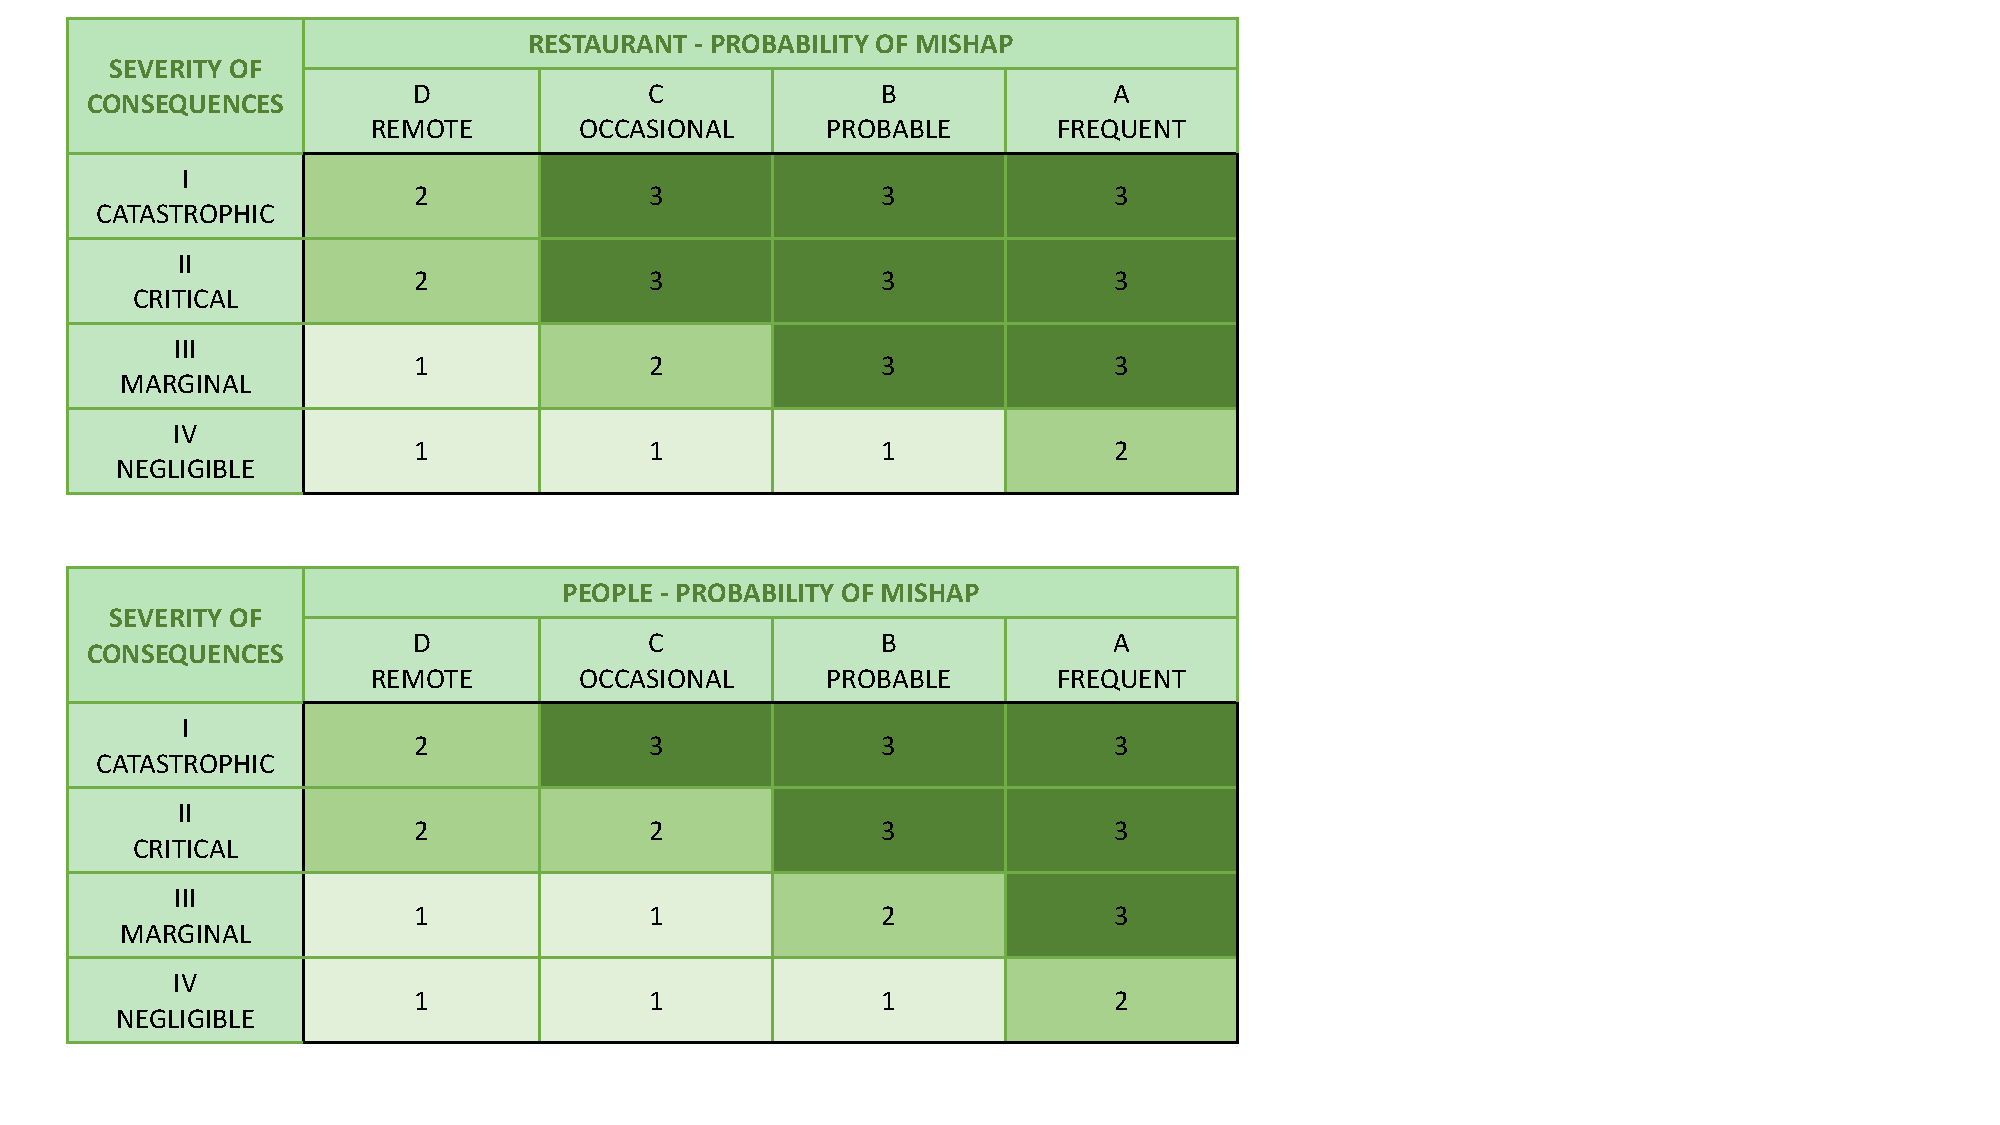
\includegraphics[height=2.7cm]{images/risk_assessment_matrix.pdf}\hspace*{1.05cm}~%
   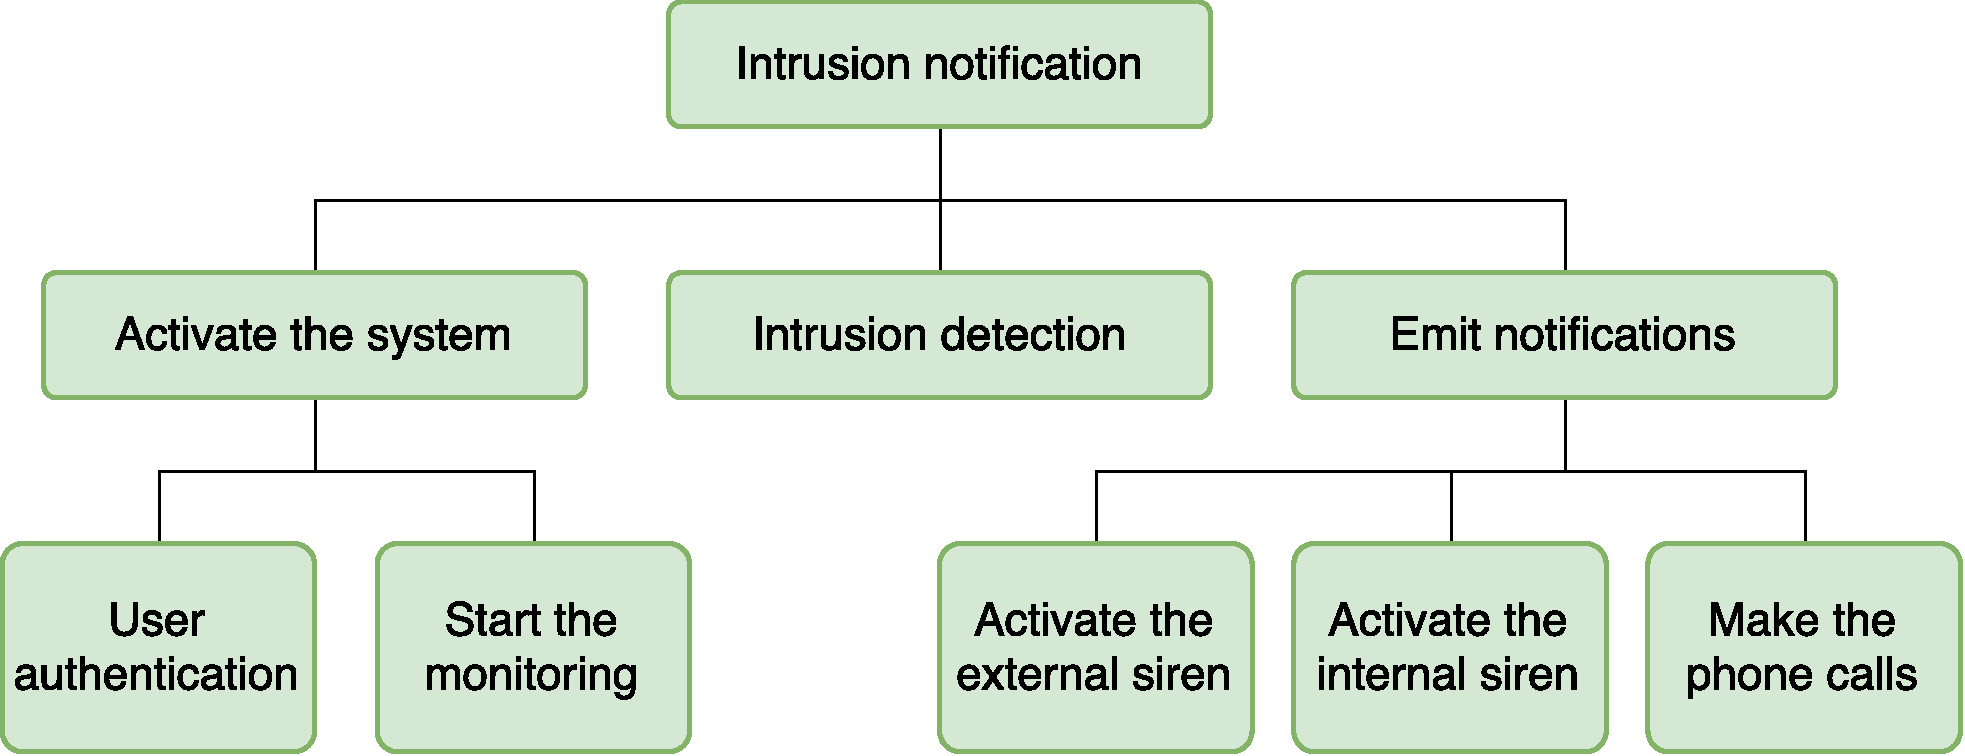
\includegraphics[width=3.5cm]{images/functional_analysis.pdf}\hspace*{0.55cm}~%
    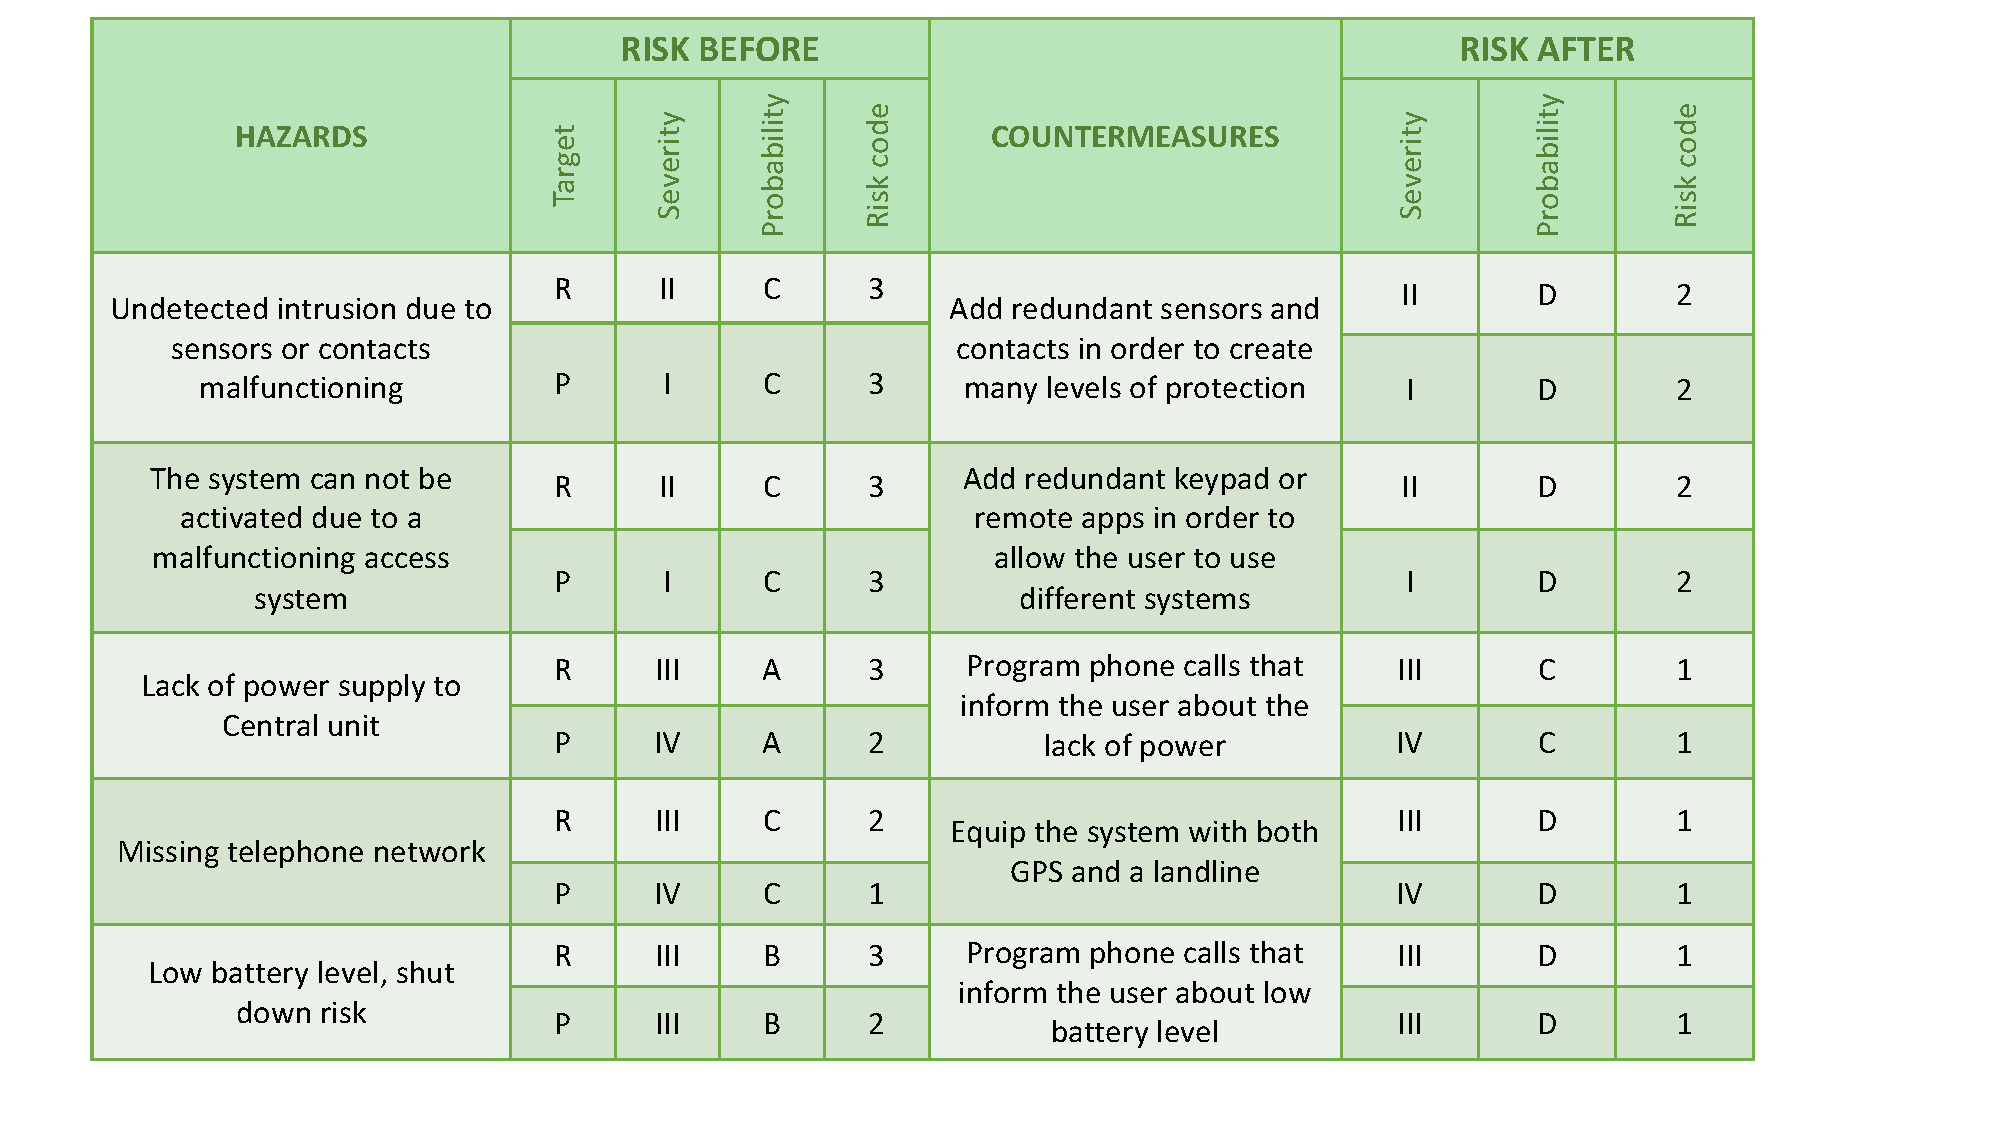
\includegraphics[height=2.3cm]{images/pha1.pdf}
}
\title[Restaurant alarm system]{\textbf{Restaurant alarm system}}
\subtitle{System Hazard Analysis}
\author[Alex Delbono]{Alex Delbono \\ }
\institute[Politecnico di Milano]{\href{mailto:alex.delbono@mail.polimi.it}{alex.delbono@mail.polimi.it}  
		\newline 
		Politecnico di Milano}
\logo{\pgfputat{\pgfxy(0,7)}{\pgfbox[right,base]{
\includegraphics[height=1.8cm]{images/logoPolimi.pdf}}}}
\date{December 4 2016}




\AtBeginSection[]
{
  \begin{frame}
    \frametitle{Table of Contents}
    \tableofcontents[currentsection]
  \end{frame}
}


%%%%%%%%%%%%%%%%%%%%%%%%   DOCUMENT   %%%%%%%%%%%%%%%%%%%%%%%
\begin{document}

%%%%%%   TITLE   %%%%%%%%%%%%
\begin{frame}
  \titlepage
\end{frame}

%%%%%% TABLE OF CONTENTS %%%%%
\begin{frame}{Overview}
\tableofcontents
\end{frame}


%%%%%% CONTENT %%%%%%%%%%
\section{System description}
\label{sec:system_description}
%%%%%%%%%%%%%%%%%%%%%%
\begin{frame}{System description}

  \begin{columns}
   \begin{column}{.50\textwidth}
  	\begin{center}
      The system we are going to analyze is a simplified example of a
      {\textcolor{green!40!black}{\fontsize{13}{15}\textbf{surveillance system}}}
      for a restaurant.

      \vskip 0.5cm

      The system must notify to the owner and to the people nearby when someone
      tries to break in and enter in the restaurant in order to steal goods or
      damage the equipment.
  	\end{center}
   \end{column}

   \begin{column}{.50\textwidth}
  	\begin{center}
      \begin{figure}[ht!]
        \centering
        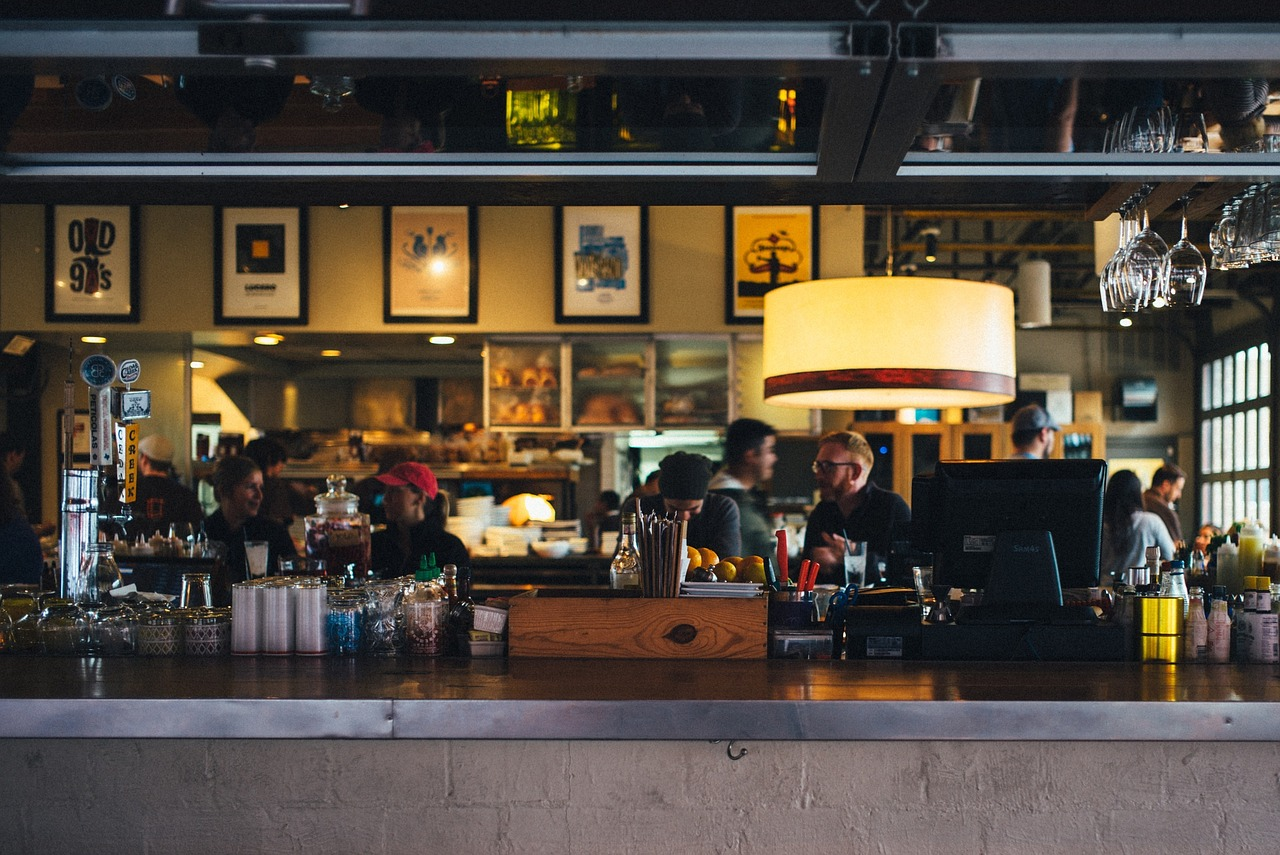
\includegraphics[width=50mm]{images/Alarm.jpg}
        \caption{Source: Alarm.org}
      \end{figure}
  	\end{center}
  	\vskip 0.3cm
   \end{column}
 \end{columns}

\end{frame}

%%%%%%%%%%%%%%%%%%%%%%
\begin{frame}{Main functions}

  \begin{columns}
   \begin{column}{.50\textwidth}
      1) The main function of the system, when active, is to signal eventual
      intruders with phone calls and acoustic signals from the sirens.

      \begin{figure}[ht!]
        \centering
        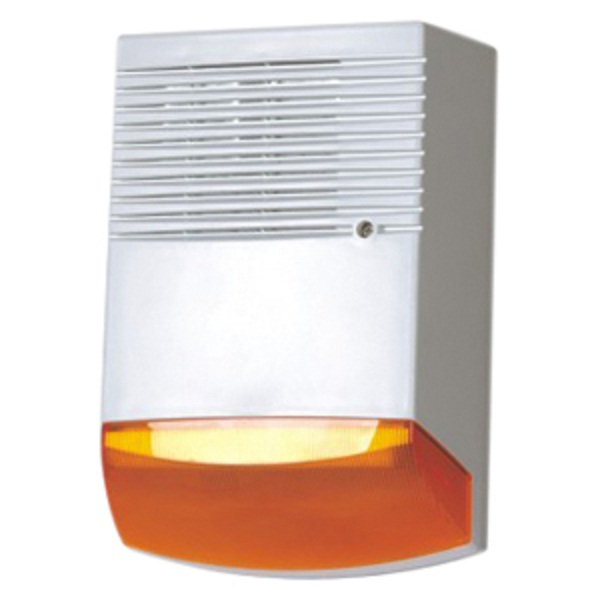
\includegraphics[width=30mm]{images/siren.jpg}
        \caption{Source: bizspia.org}
      \end{figure}

   \end{column}

   \begin{column}{.50\textwidth}
   \vskip 0.1cm

   \begin{figure}[ht!]
     \centering
     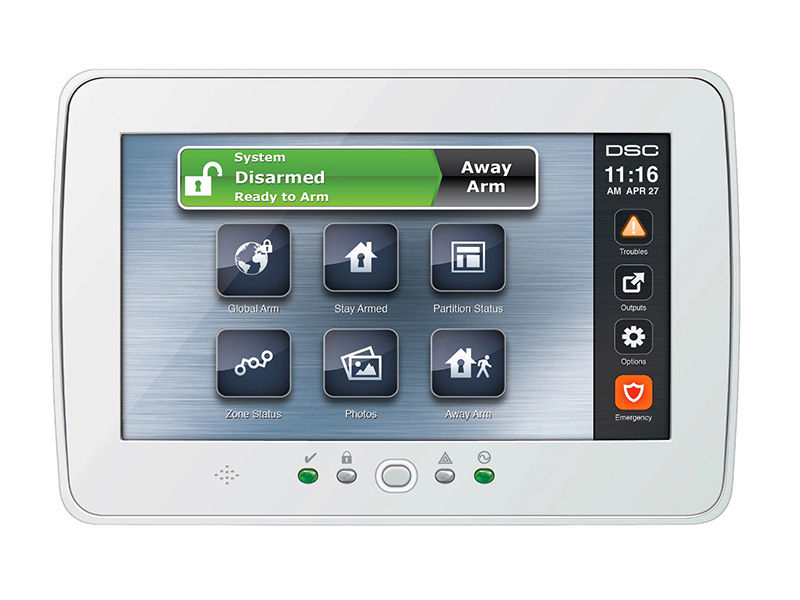
\includegraphics[width=30mm]{images/dsc.jpg}
     \caption{Source: dsc.com}
   \end{figure}

   \vskip 0.1cm
   2) It must be possible for authorized people to disable the system,
   either locally or using a remote procedure.
   \end{column}
 \end{columns}

\end{frame}

%%%%%%%%%%%%%%%%%%%%%%
\begin{frame}{Focus of the analysis}

  \begin{columns}
   \begin{column}{.50\textwidth}
      The objective of the analysis is to provide a description
      of the system hazards from an
      {\textcolor{green!40!black}{\fontsize{13}{15}\textbf{high level point of view}}},
      considering the main components as atomic.

      \vskip 0.8cm

      In this way we avoid the complexity of the analysis of the subcomponents,
      but we can focus only on the functionalities offered to the users.

   \end{column}

   \begin{column}{.50\textwidth}
   \vskip 0.3cm

   \begin{figure}[ht!]
     \centering
     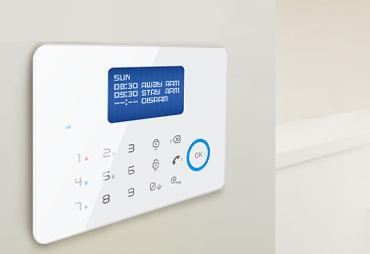
\includegraphics[width=50mm]{images/keypad.jpg}
     \caption{Source: DHgate.com}
   \end{figure}

   \end{column}
 \end{columns}

\end{frame}

%%%%%%%%%%%%%%%%%%%%%%
\begin{frame}{General system overview}

  \begin{columns}
   \begin{column}{.50\textwidth}
      The {\textcolor{green!40!black}{\fontsize{13}{15}\textbf{main}}}
       hardware and software
       {\textcolor{green!40!black}{\fontsize{13}{15}\textbf{components}}}
        of the system are presented
      in the following list:
      \begin{itemize}
        \item Central unit
        \item Infrared sensors
        \item Magnetic contacts
        \item Internal and external sirens
        \item Telephone module
        \item Alarm module
        \item Output modules
        \item User access points
      \end{itemize}
   \end{column}

   \begin{column}{.50\textwidth}
   \vskip 0.3cm
   \begin{center}
      \begin{figure}[ht!]
        \centering
        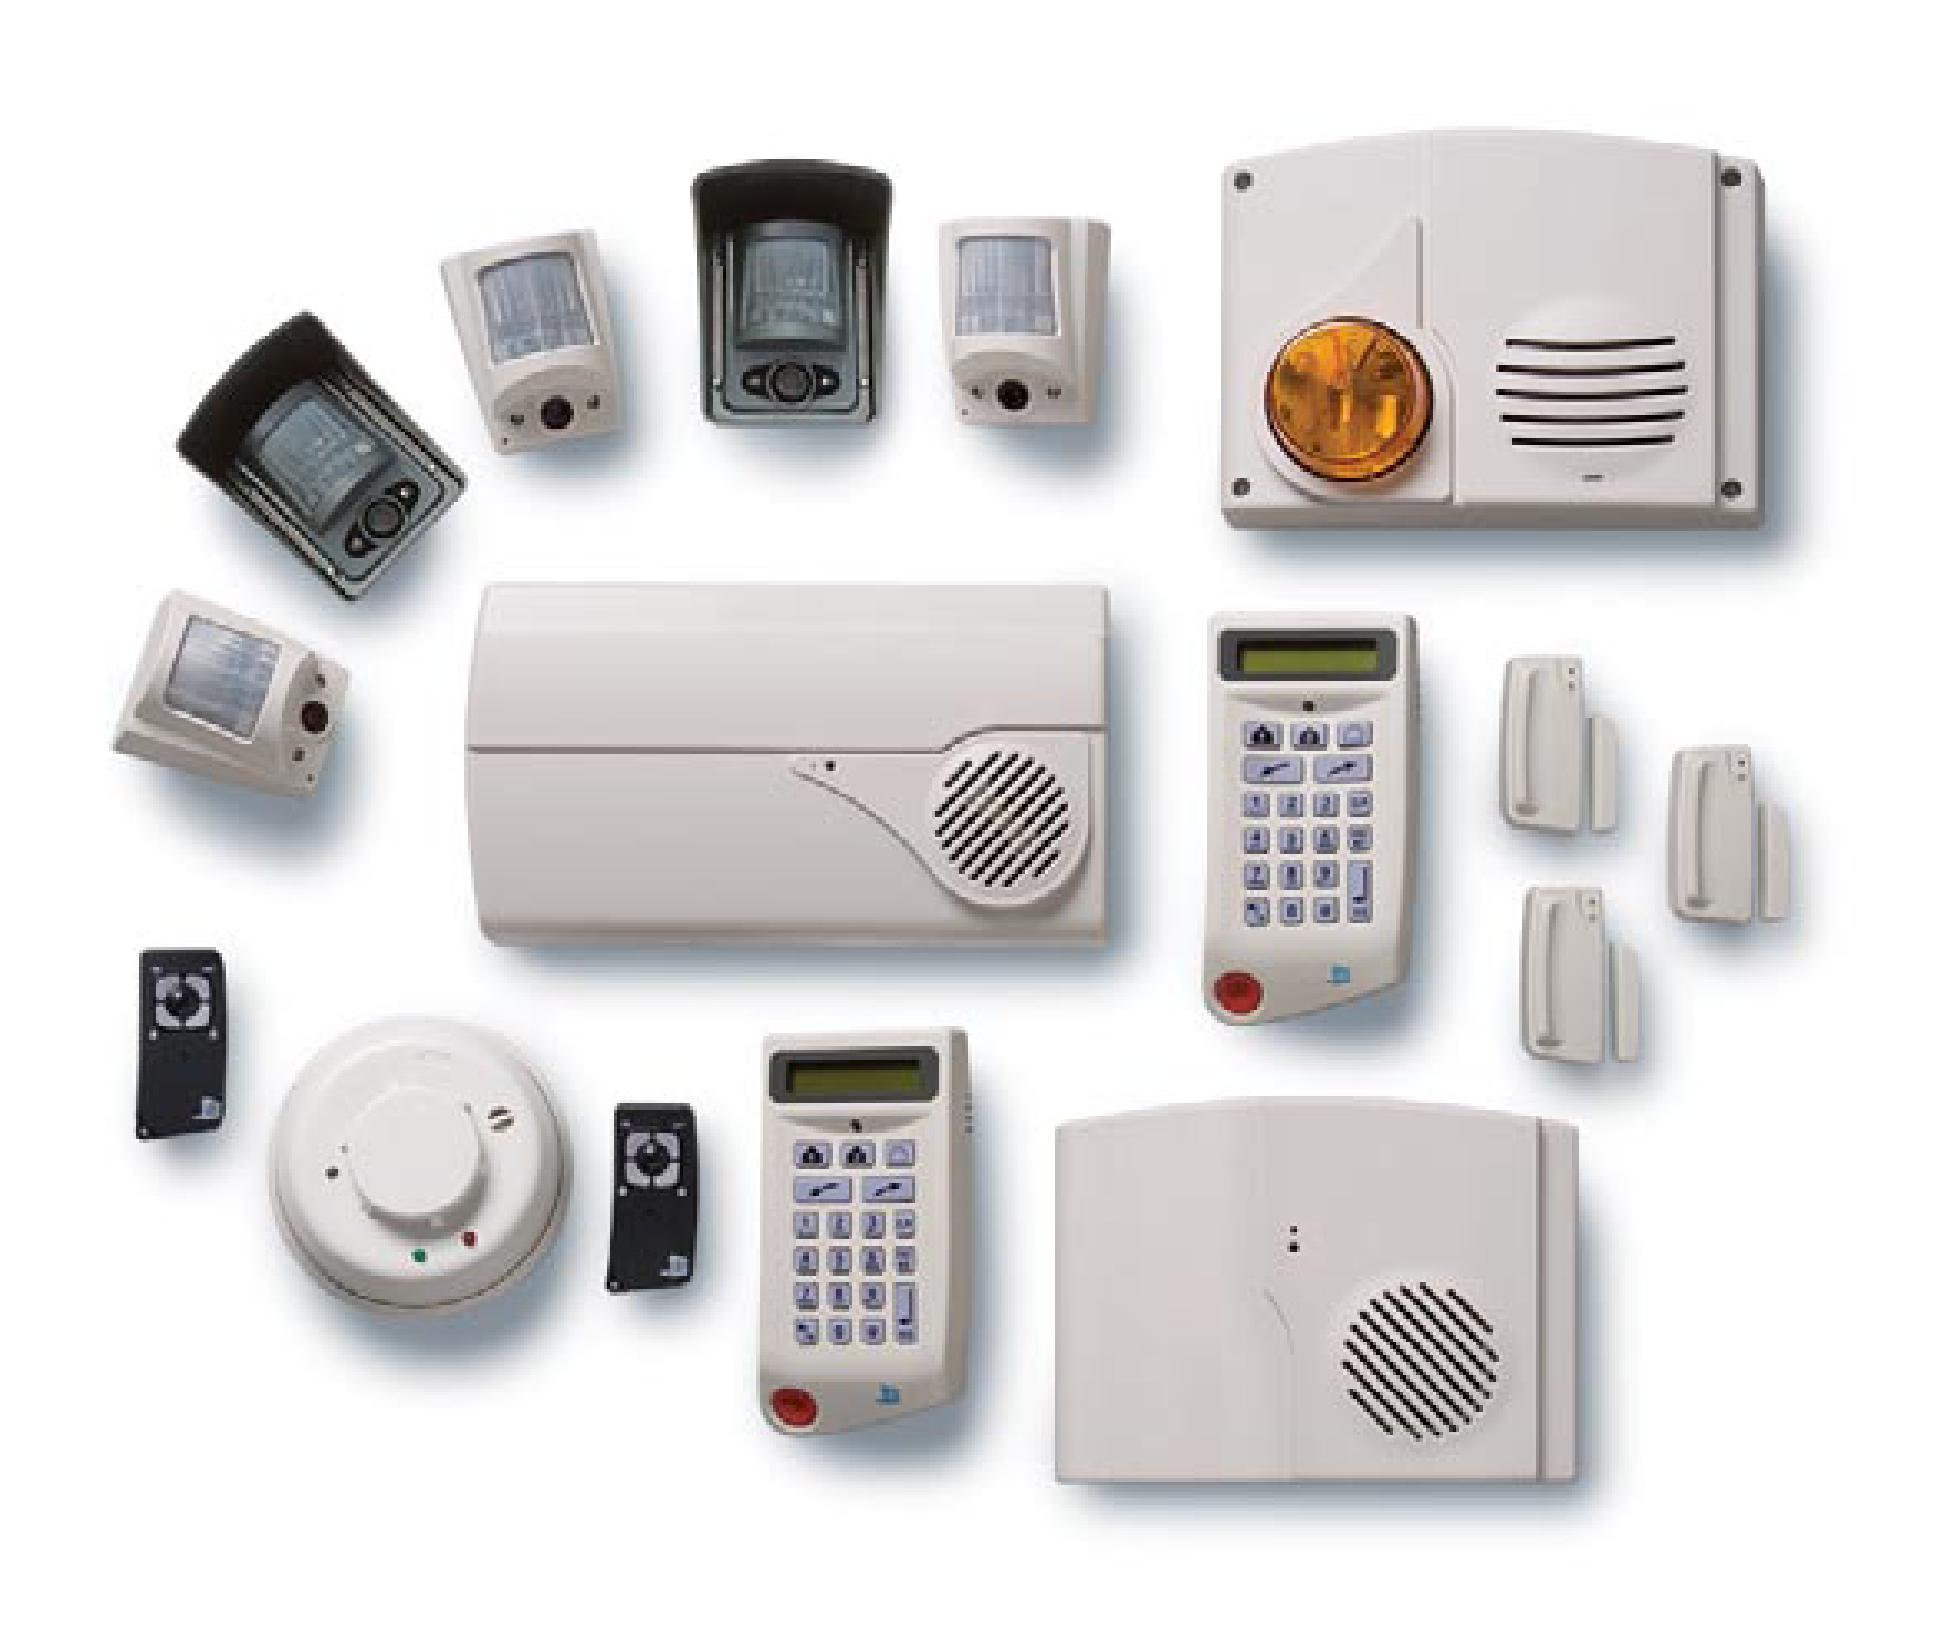
\includegraphics[width=60mm]{images/alarm_systems.jpg}
        \caption{Source: coreportal.org}
      \end{figure}
   \end{center}
   \end{column}
 \end{columns}

\end{frame}

%%%%%%%%%%%%%%%%%%%%%%
\begin{frame}{Components}

  \begin{columns}
   \begin{column}{.50\textwidth}
    The {\textcolor{green!40!black}{\fontsize{13}{15}\textbf{Central unit}}}
    controls all the system and offers the power supply to all the components.
      \vskip 0.3cm

    The {\textcolor{green!40!black}{\fontsize{13}{15}\textbf{infrared sensors
    and the magnetic contacts}}}
    protect the openings and the rooms of the building.
      \vskip 0.3cm

    The {\textcolor{green!40!black}{\fontsize{13}{15}\textbf{two sirens}}},
    one internal and one external, signal a perceived intrusion through
    acoustic advices.

      \vskip 0.3cm

    The {\textcolor{green!40!black}{\fontsize{13}{15}\textbf{telephone module}}}
    is in charge to make phone calls whenever an alarm is detected.

   \end{column}

   \begin{column}{.50\textwidth}
    The {\textcolor{green!40!black}{\fontsize{13}{15}\textbf{alarm module}}}
    receives the perceptions of the sensors and decides whether there is
    an intrusion or not. It also communicates with the sirens and
    the telephone module.

     \vskip 0.3cm

    The {\textcolor{green!40!black}{\fontsize{13}{15}\textbf{output module}}}
    informs the user about the state of the system, using leds.

     \vskip 0.3cm

    The {\textcolor{green!40!black}{\fontsize{13}{15}\textbf{user access points}}}
    allow the user to login and change the state of the system.
   \end{column}
 \end{columns}

\end{frame}


\section{Functional analysis}
\label{sec:functional_analysis}
%%%%%%%%%%%%%%%%%%%%%%
\begin{frame}{Functional analysis}

  \begin{figure}[ht!]
    \centering
    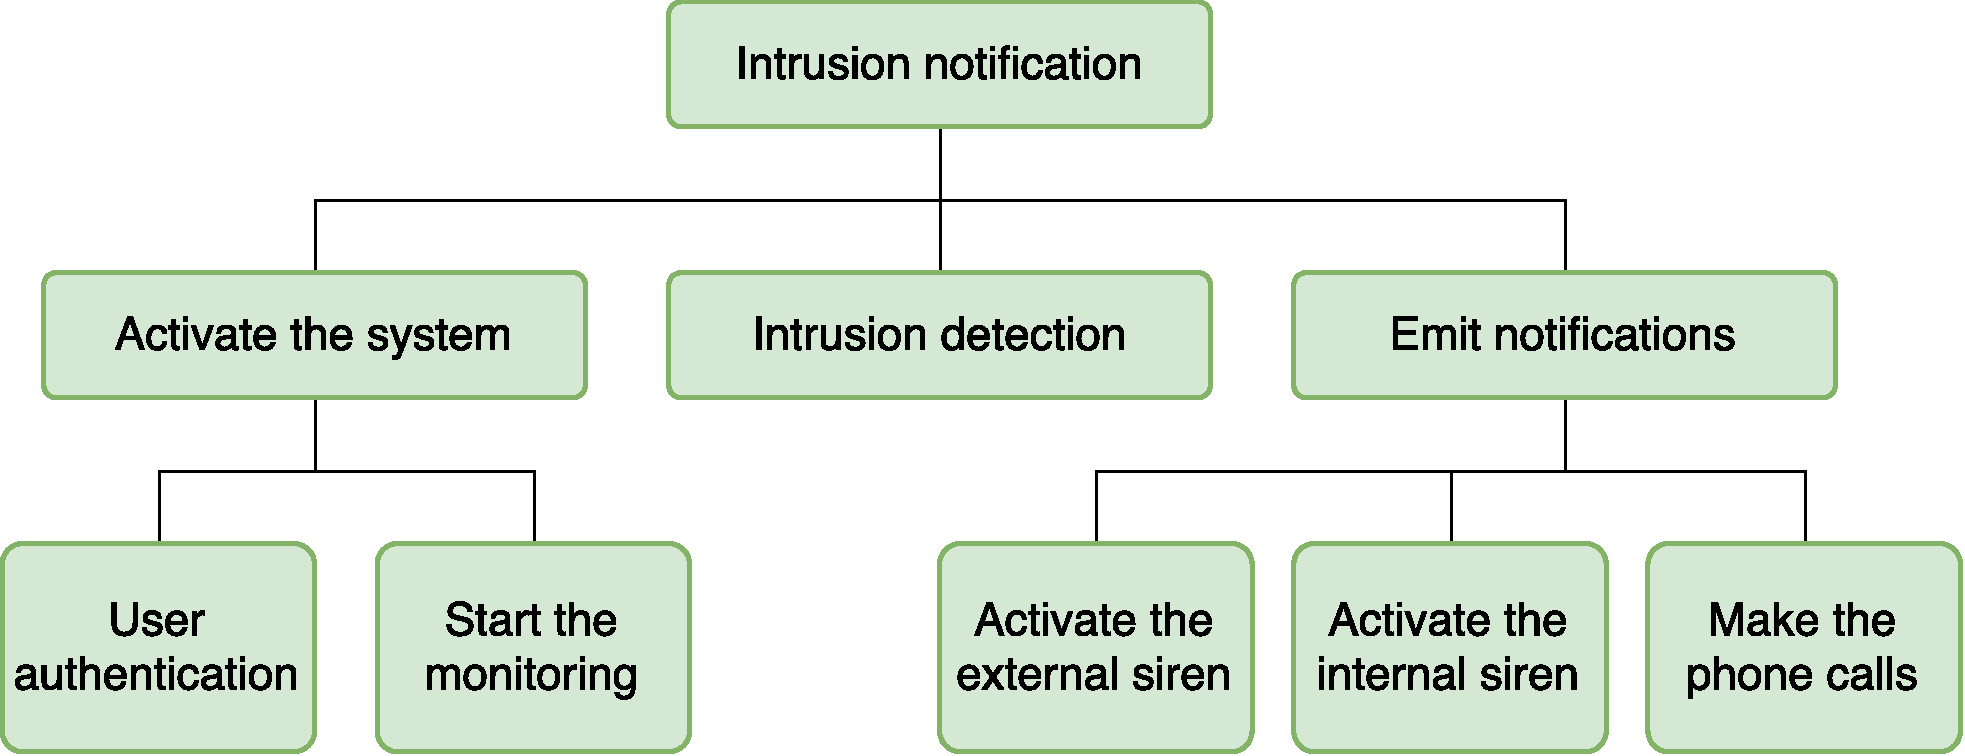
\includegraphics[width=120mm]{images/functional_analysis.pdf}
    \label{fig:functional_analysis}
  \end{figure}

\end{frame}


\section{Architectural analysis}
\label{sec:architectural_analysis}
%%%%%%%%%%%%%%%%%%%%%%
\begin{frame}{Architectural analysis}

  \begin{figure}[ht!]
    \centering
    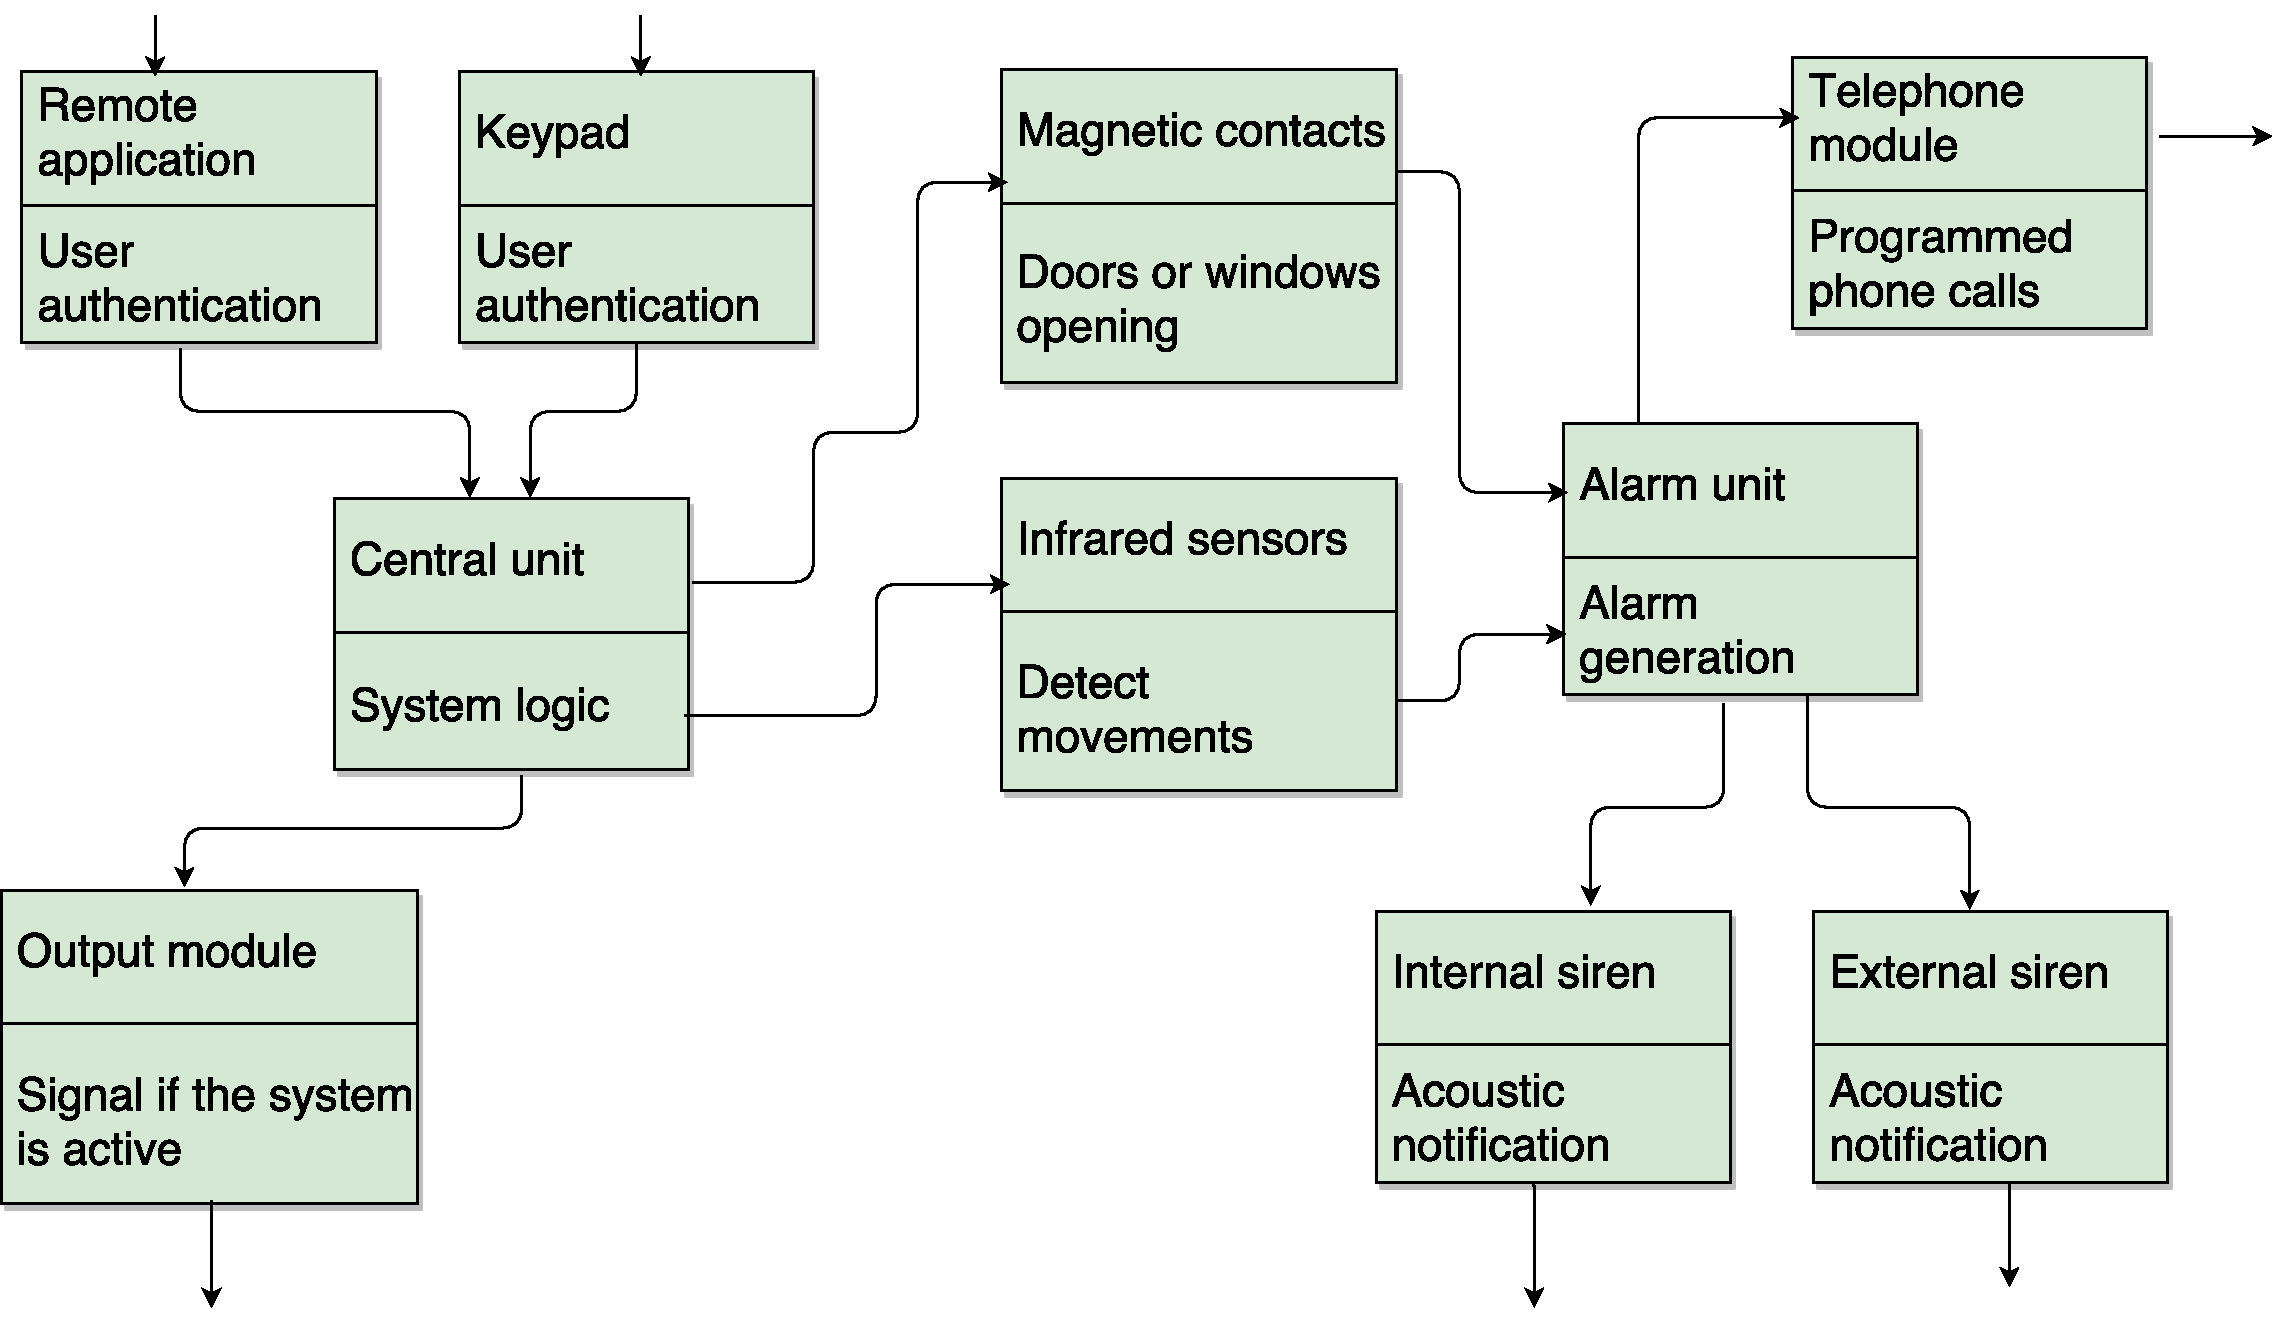
\includegraphics[width=120mm]{images/architectural_analysis.pdf}
    \label{fig:architectural_analysis}
  \end{figure}

\end{frame}


\section{Qualitative analysis (PHA)}
\label{sec:qualitative_analysis}
%%%%%%%%%%%%%%%%%%%%%%
\begin{frame}{PHA - Operating modes}
\vskip 0.9cm
    \begin{figure}[ht!]
      \centering
      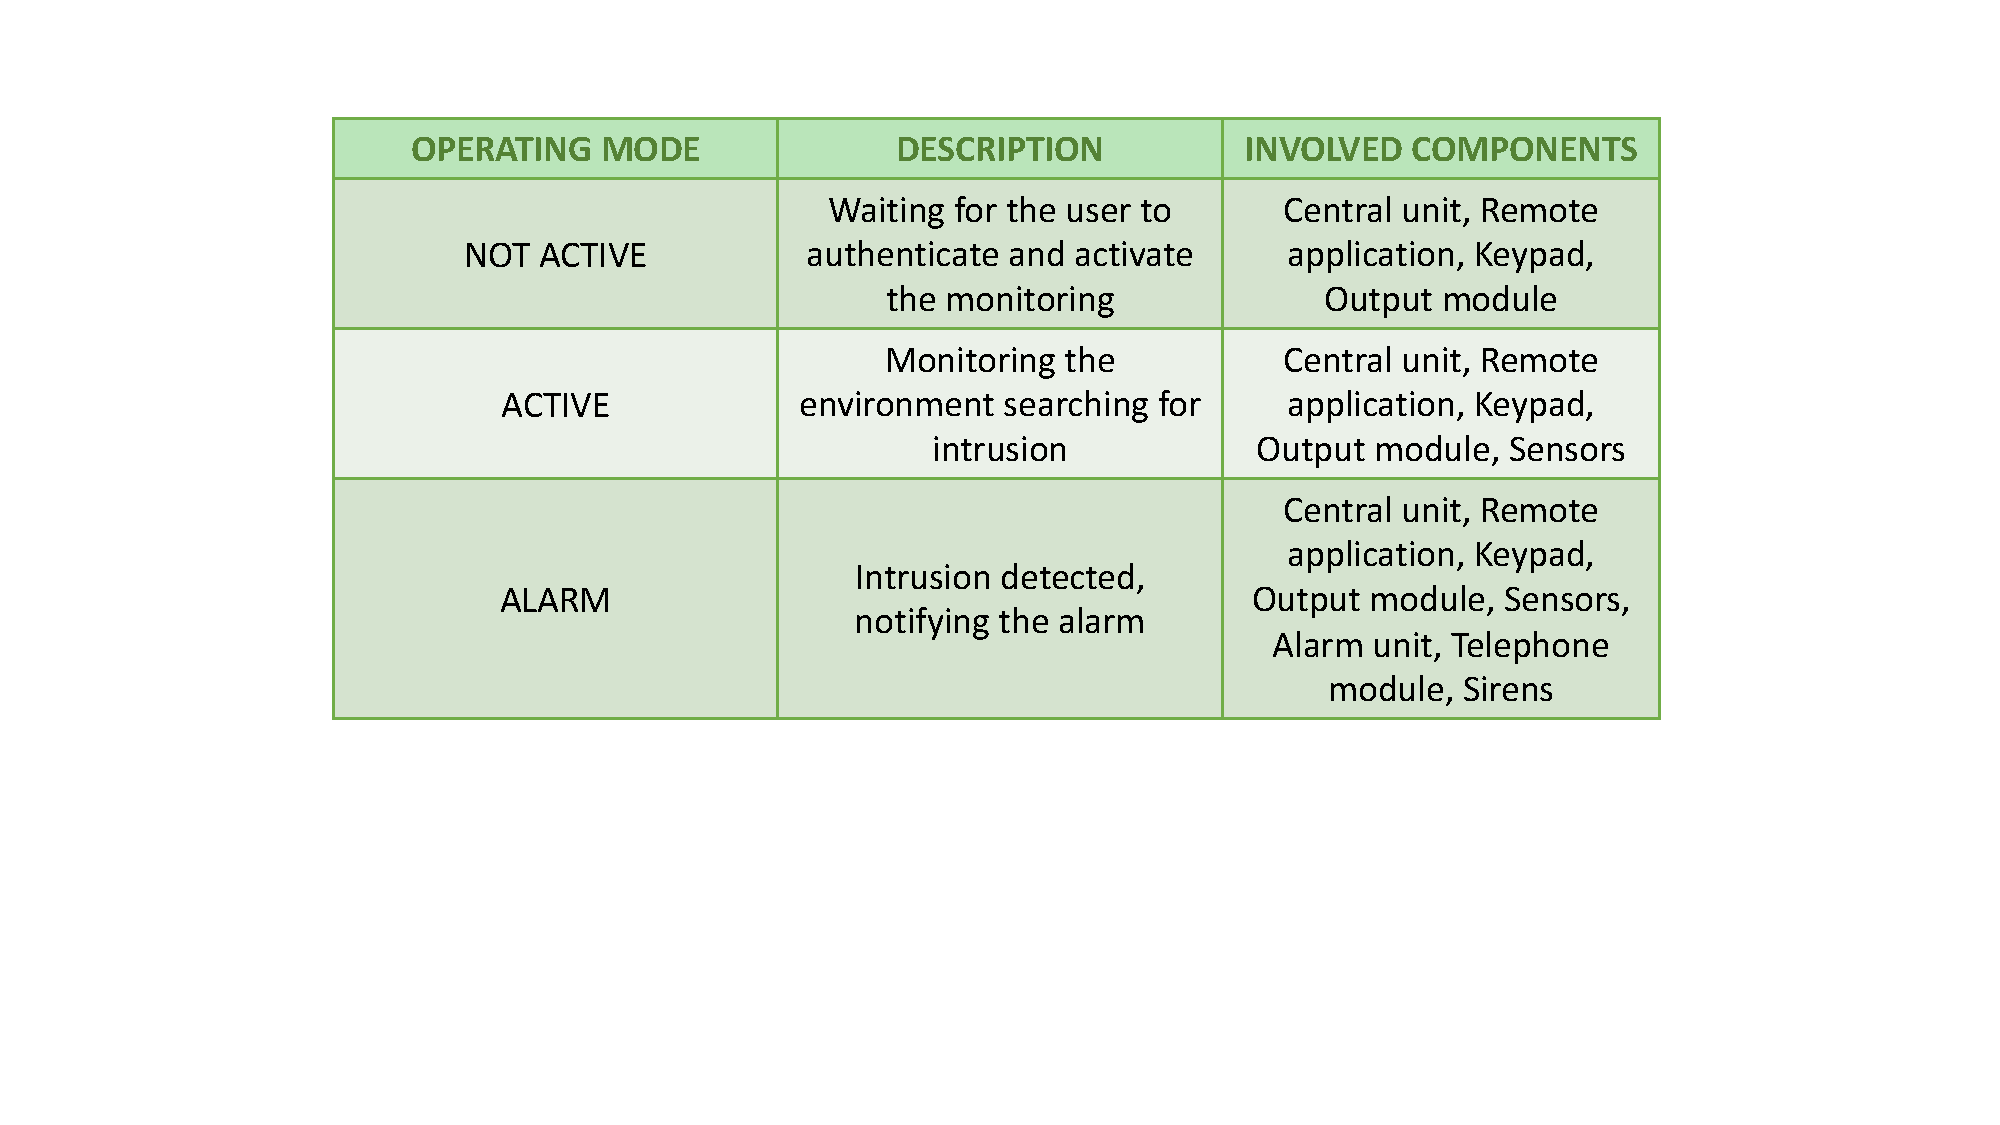
\includegraphics[width=120mm]{images/operating_modes.pdf}
      \label{fig:operating_modes}
    \end{figure}
\end{frame}

%%%%%%%%%%%%%%%%%%%%%%
\begin{frame}{PHA - Hazard description (1)}
\vskip 0.9cm
    \begin{figure}[ht!]
      \centering
      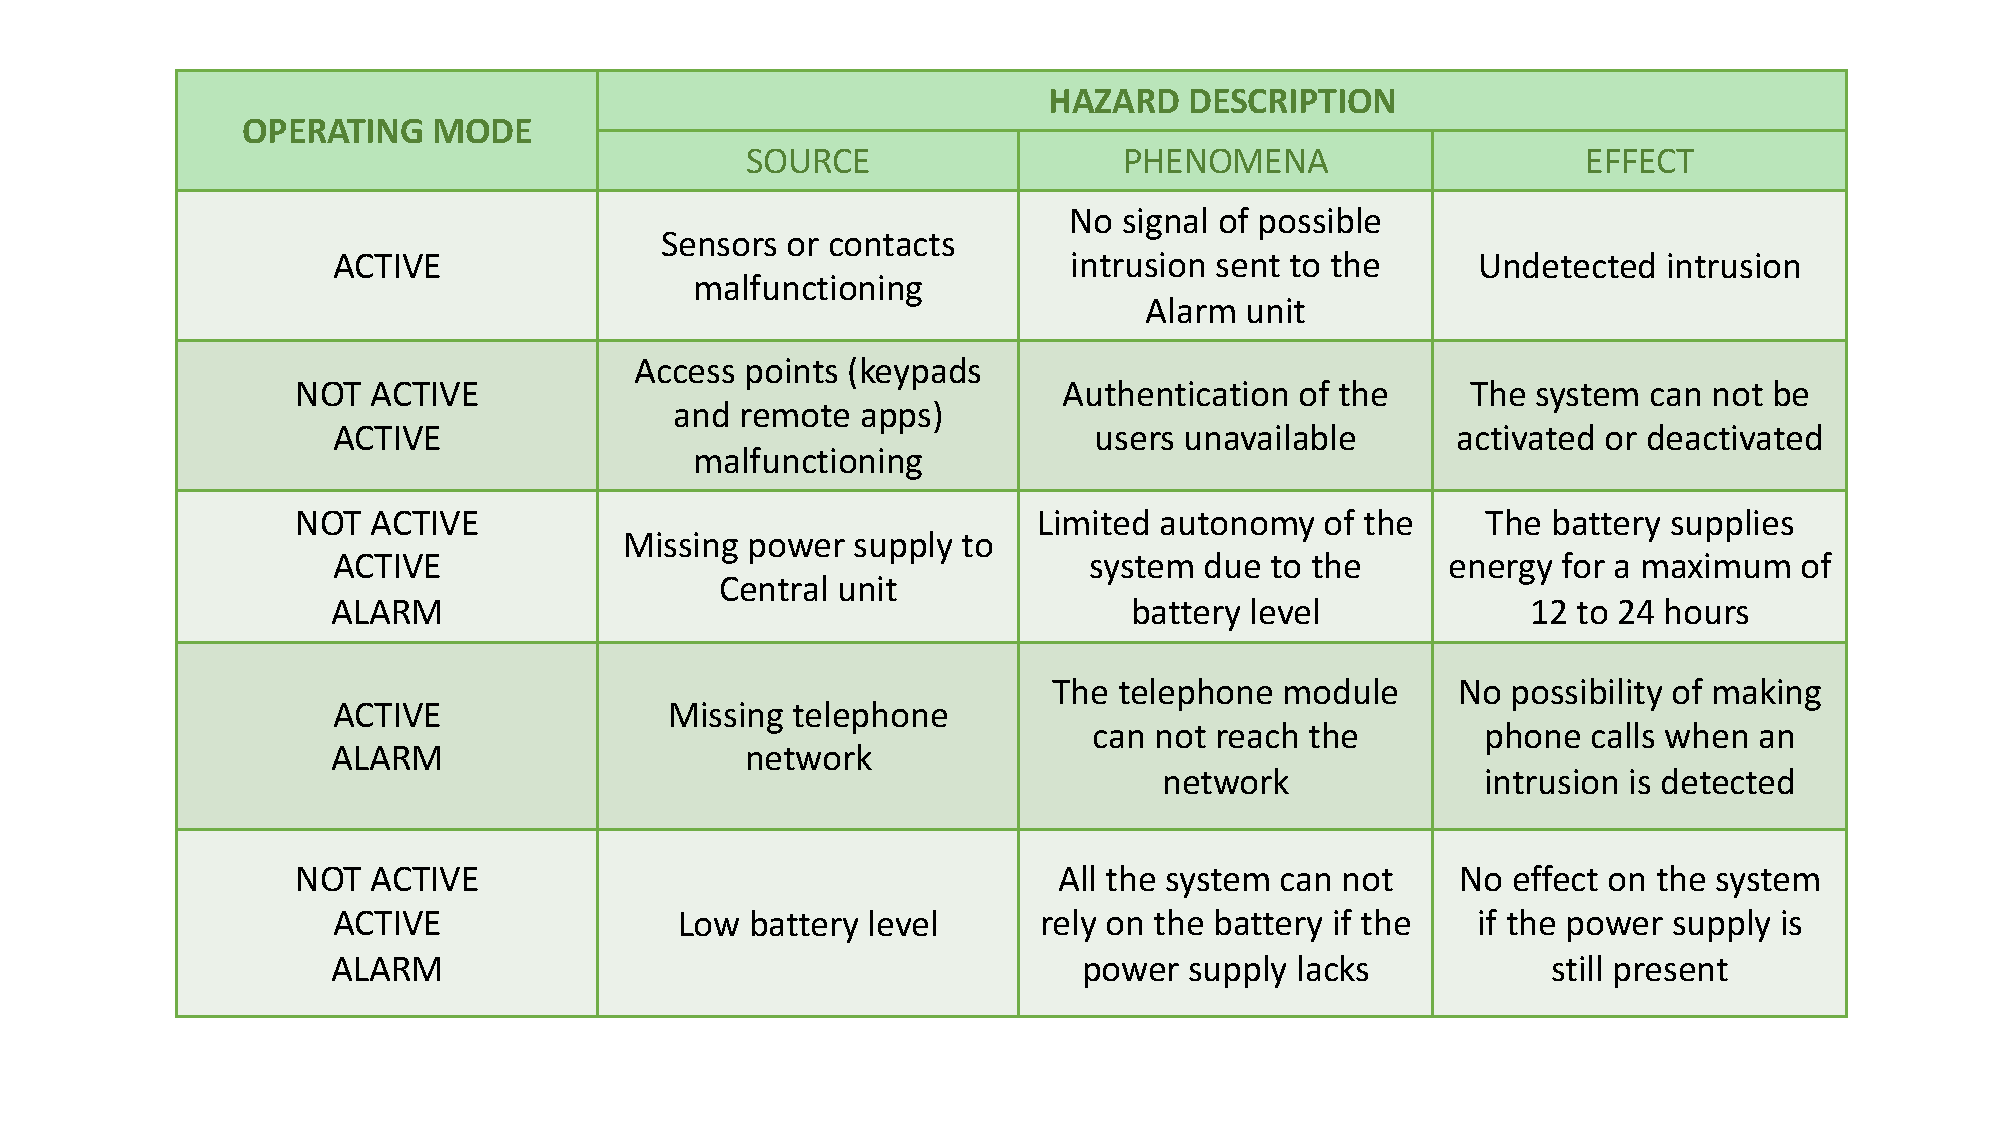
\includegraphics[width=120mm]{images/hazard_description1.pdf}
      \label{fig:hazard_description}
    \end{figure}
\end{frame}

%%%%%%%%%%%%%%%%%%%%%%
\begin{frame}{PHA - Hazard description (2)}
\vskip 0.9cm
    \begin{figure}[ht!]
      \centering
      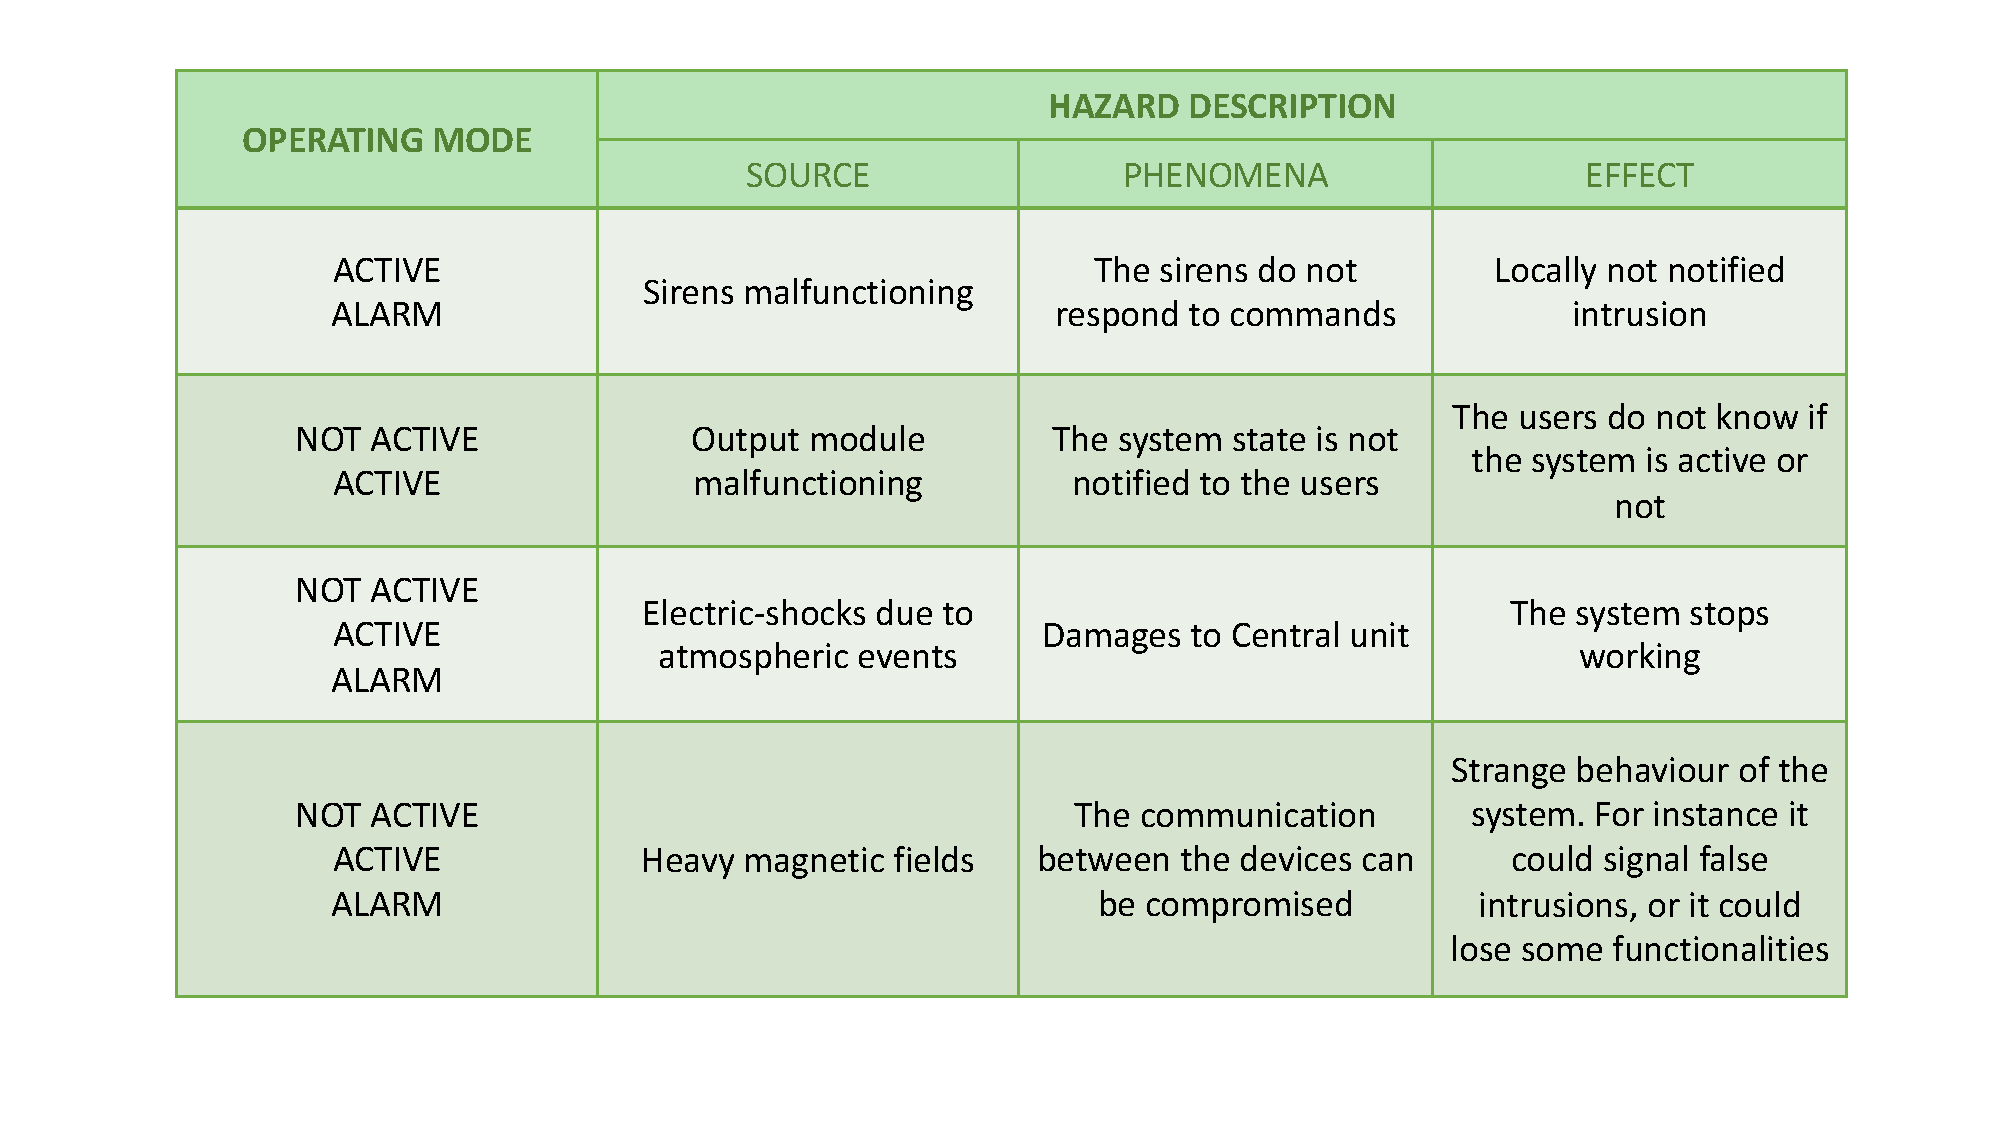
\includegraphics[width=120mm]{images/hazard_description2.pdf}
    \end{figure}
\end{frame}

%%%%%%%%%%%%%%%%%%%%%%
\begin{frame}{PHA - Targets}
\vskip 0.9cm
    \begin{figure}[ht!]
      \centering
      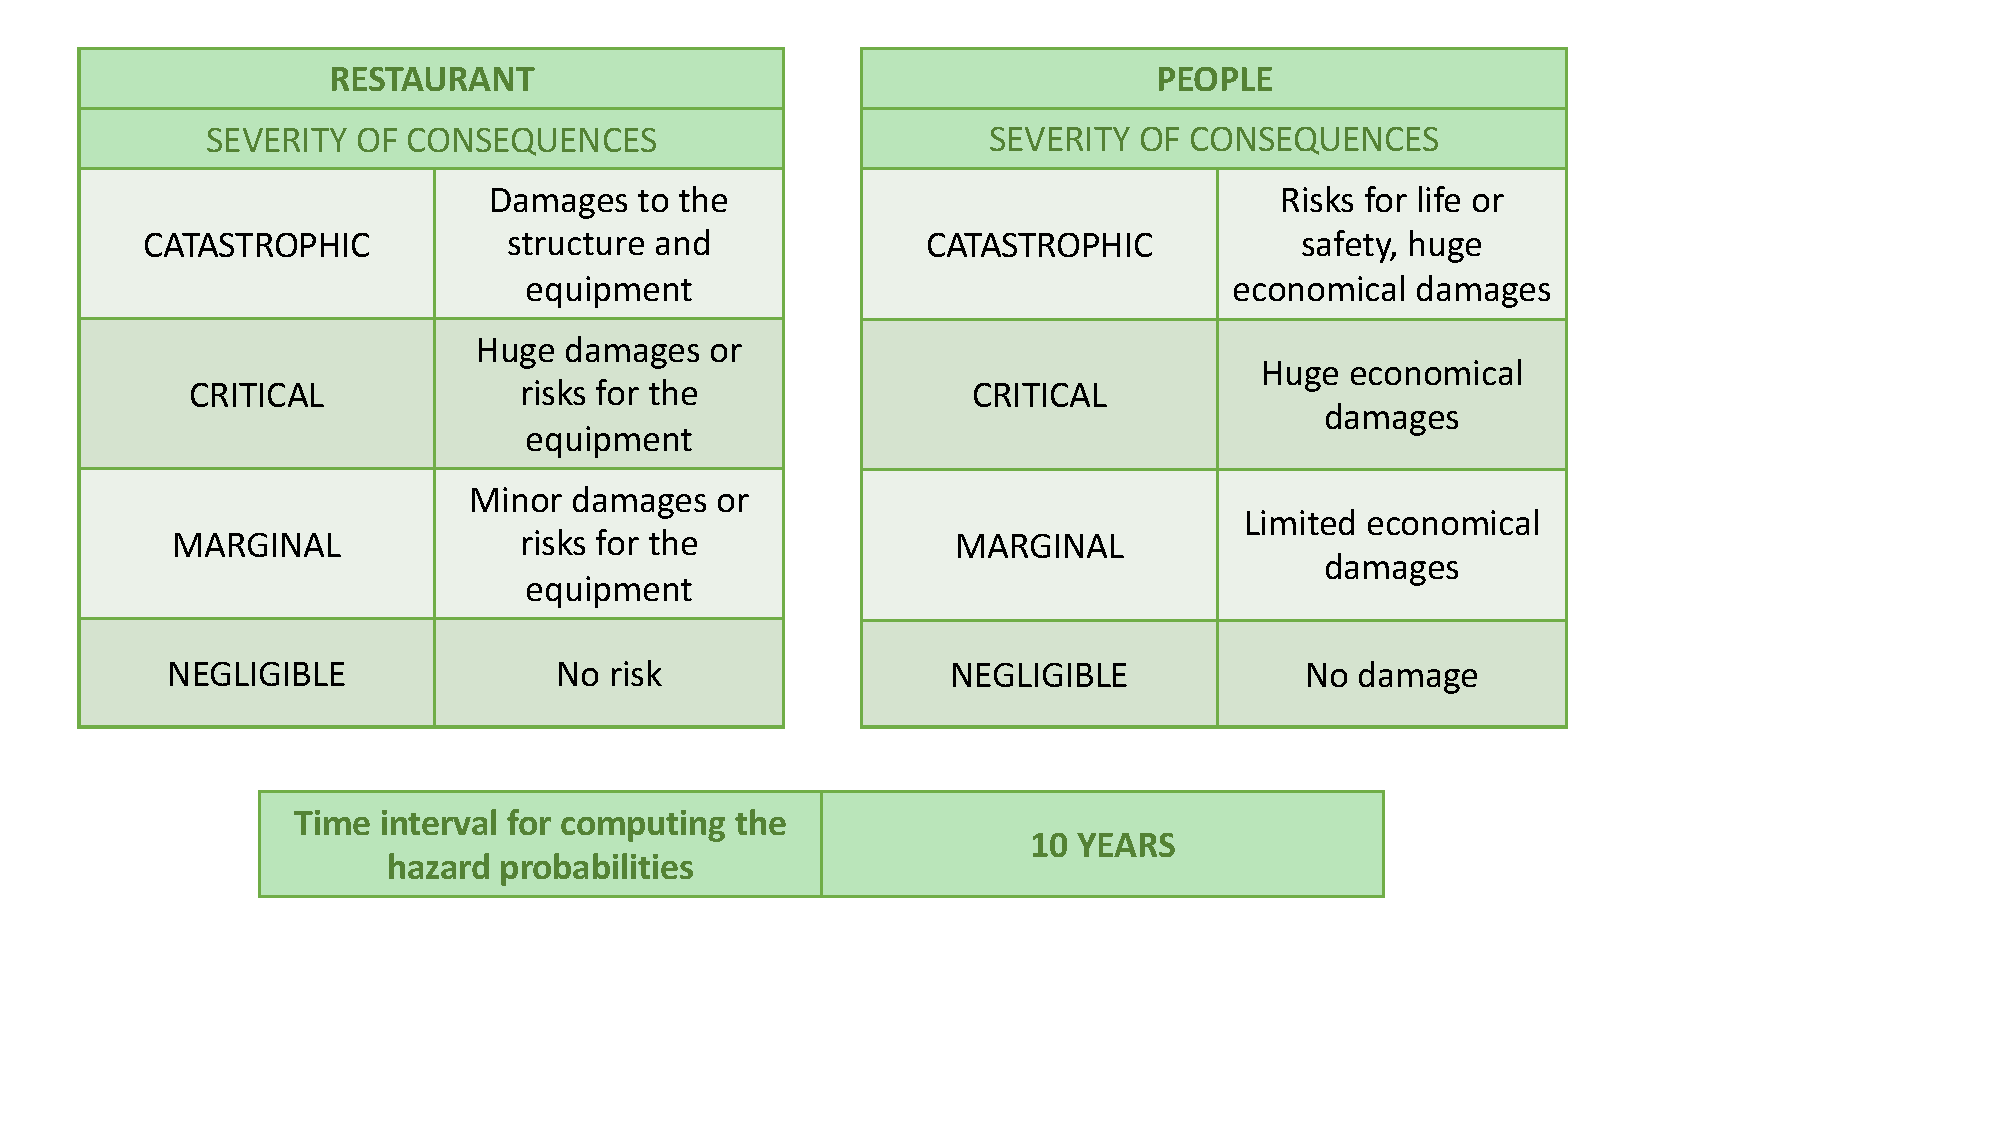
\includegraphics[width=120mm]{images/targets.pdf}
      \label{fig:targets}
    \end{figure}
\end{frame}

%%%%%%%%%%%%%%%%%%%%%%
\begin{frame}{PHA - Risk assessment matrixes}

    \begin{figure}[ht!]
      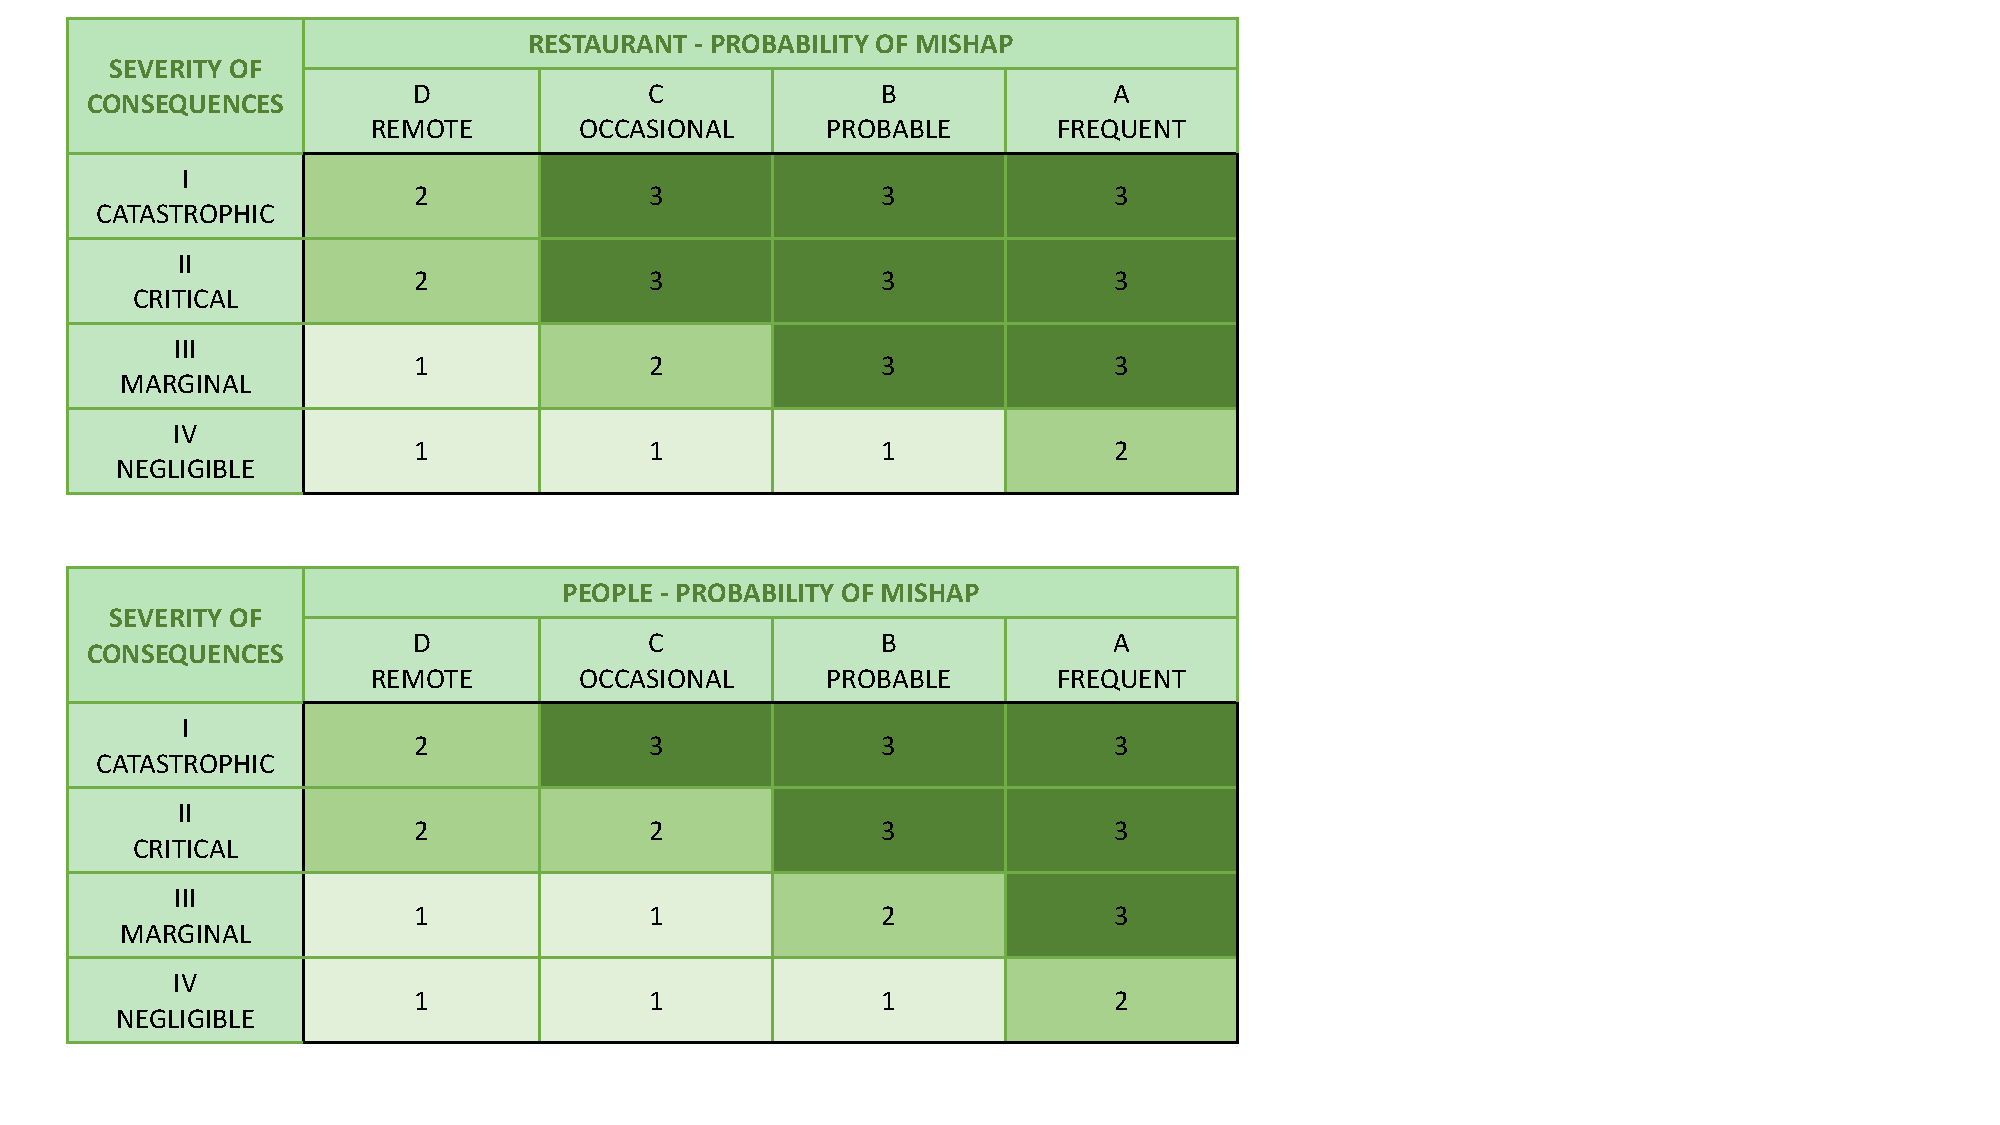
\includegraphics[width=80mm]{images/risk_assessment_matrix.pdf}
      \label{fig:risk_assessment_matrix}
    \end{figure}
\end{frame}

%%%%%%%%%%%%%%%%%%%%%%
\begin{frame}{PHA (1)}
  \vskip 0.7cm
    \begin{figure}[ht!]
      \centering
      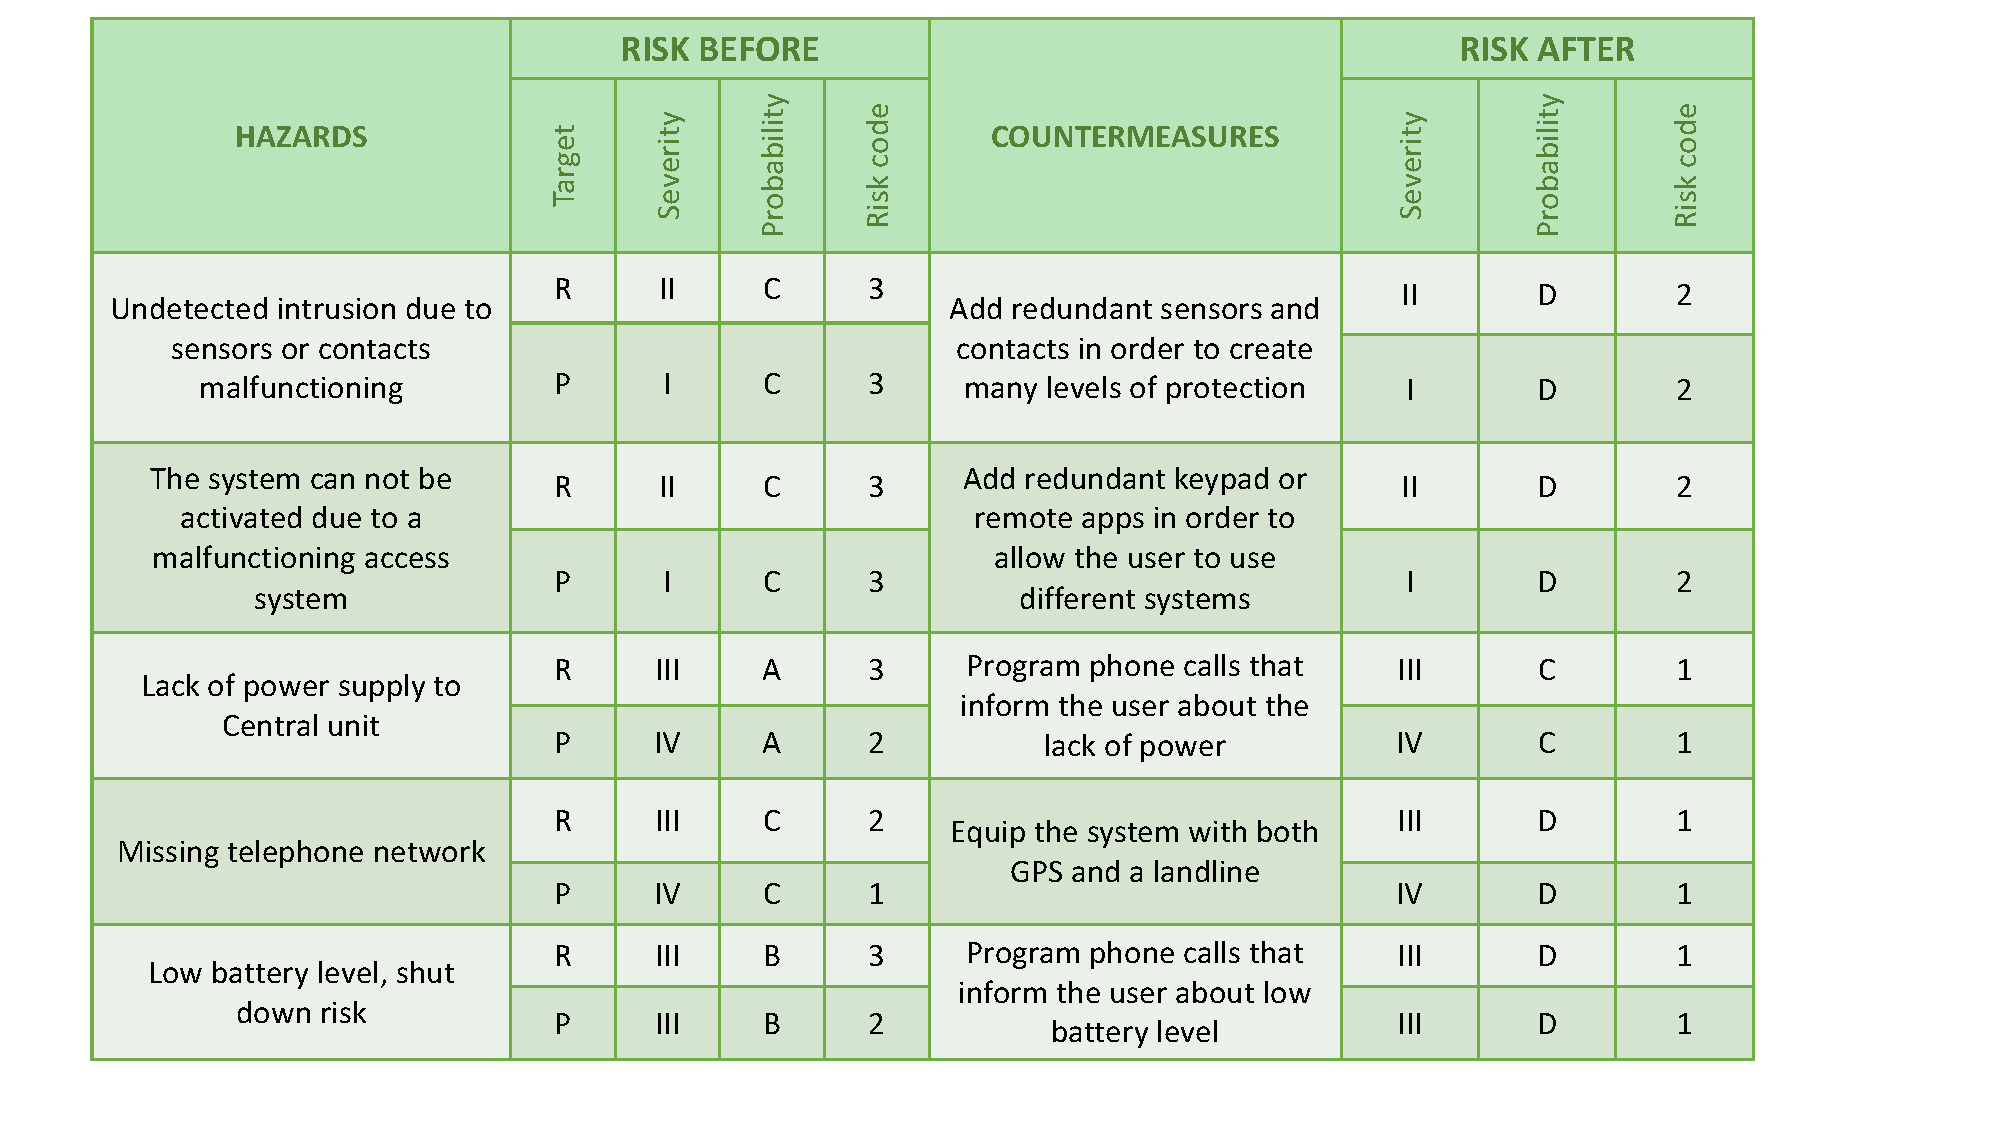
\includegraphics[width=110mm]{images/pha1.pdf}
      \label{fig:pha1}
    \end{figure}
\end{frame}

%%%%%%%%%%%%%%%%%%%%%%
\begin{frame}{PHA (2)}
  \vskip 0.6cm
    \begin{figure}[ht!]
      \centering
      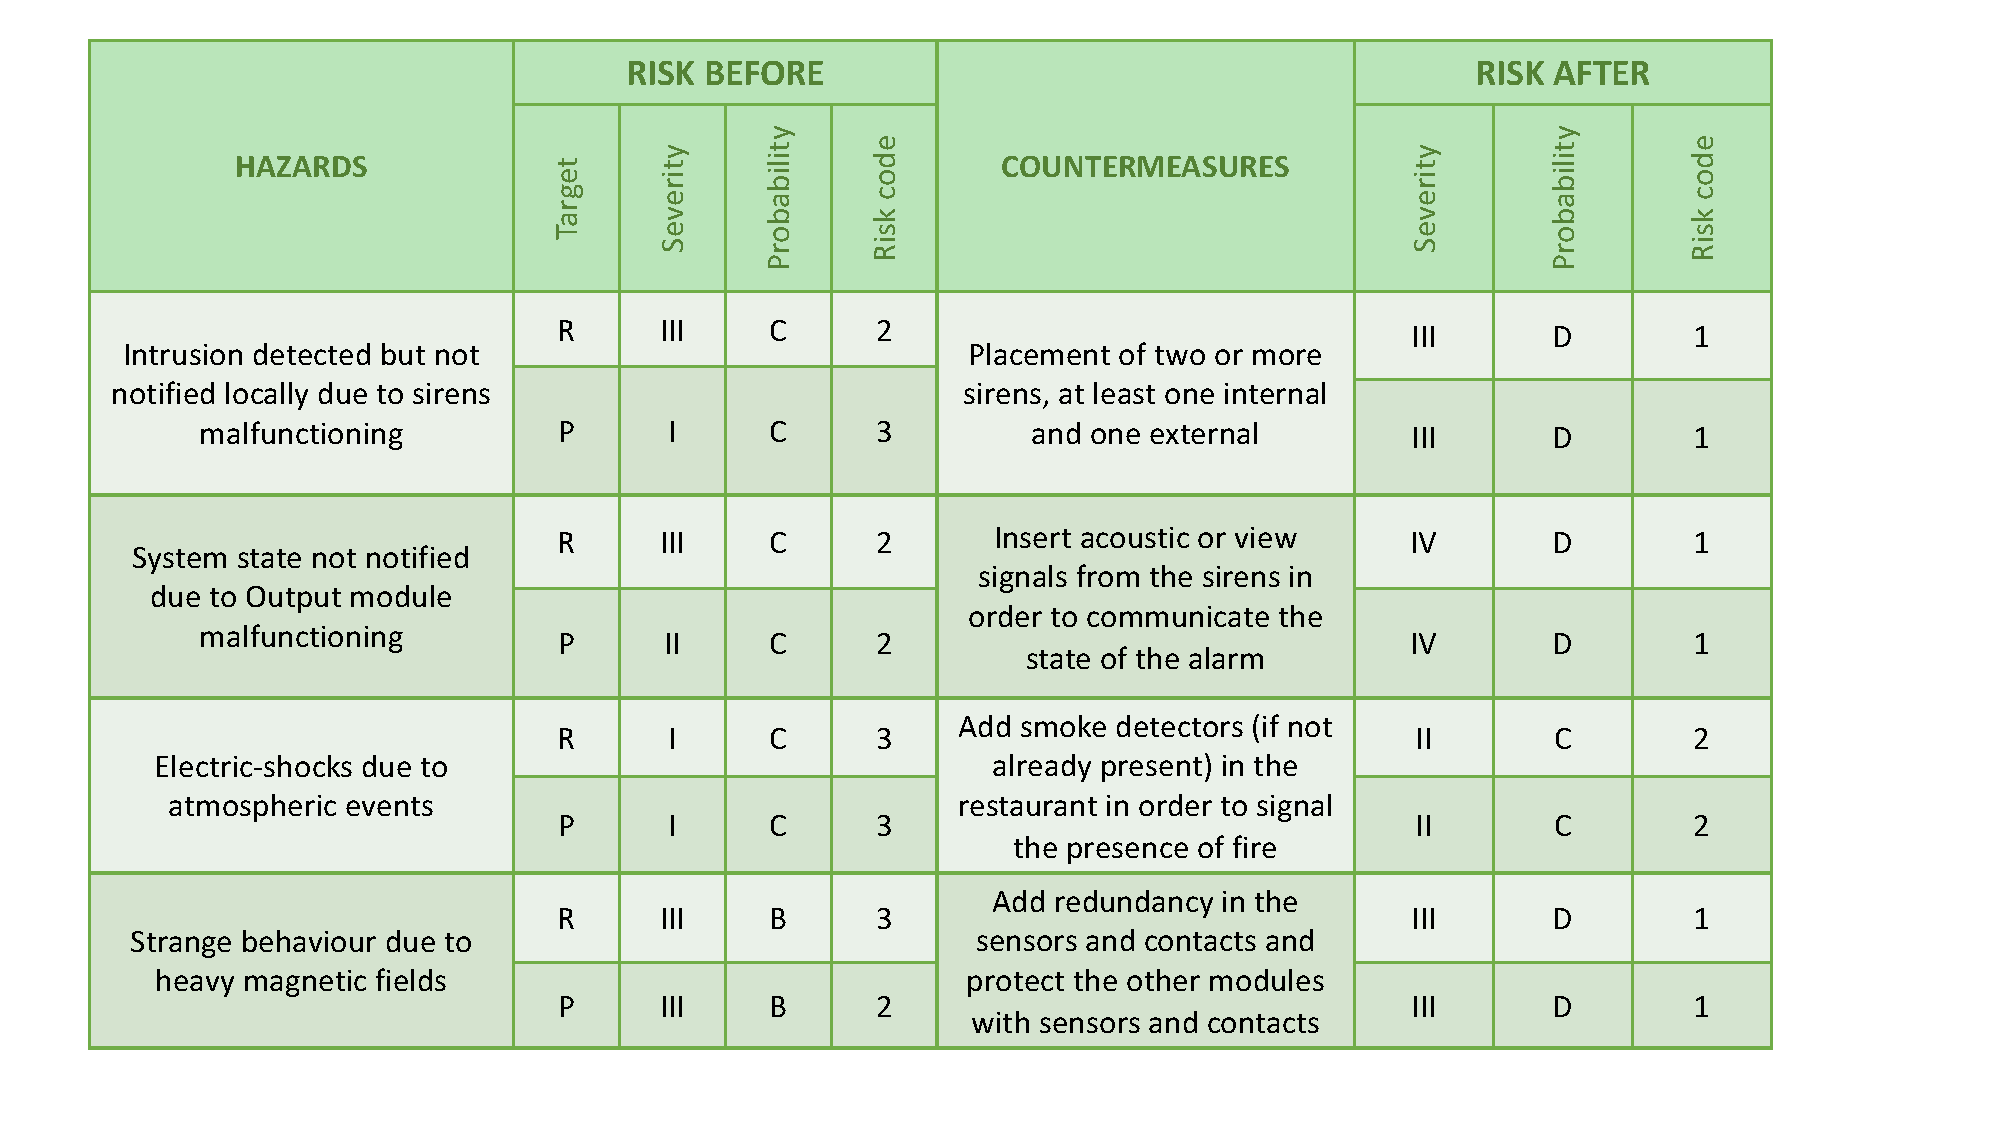
\includegraphics[width=110mm]{images/pha2.pdf}
      \label{fig:pha2}
    \end{figure}
\end{frame}


\section{Quantitative analysis}
\label{sec:quantitative_analysis}
\subsection{FMEA}
\label{sec:fmea}
%%%%%%%%%%%%%%%%%%%%%%
\begin{frame}{FMEA - Structure definition}

    \begin{figure}[ht!]
      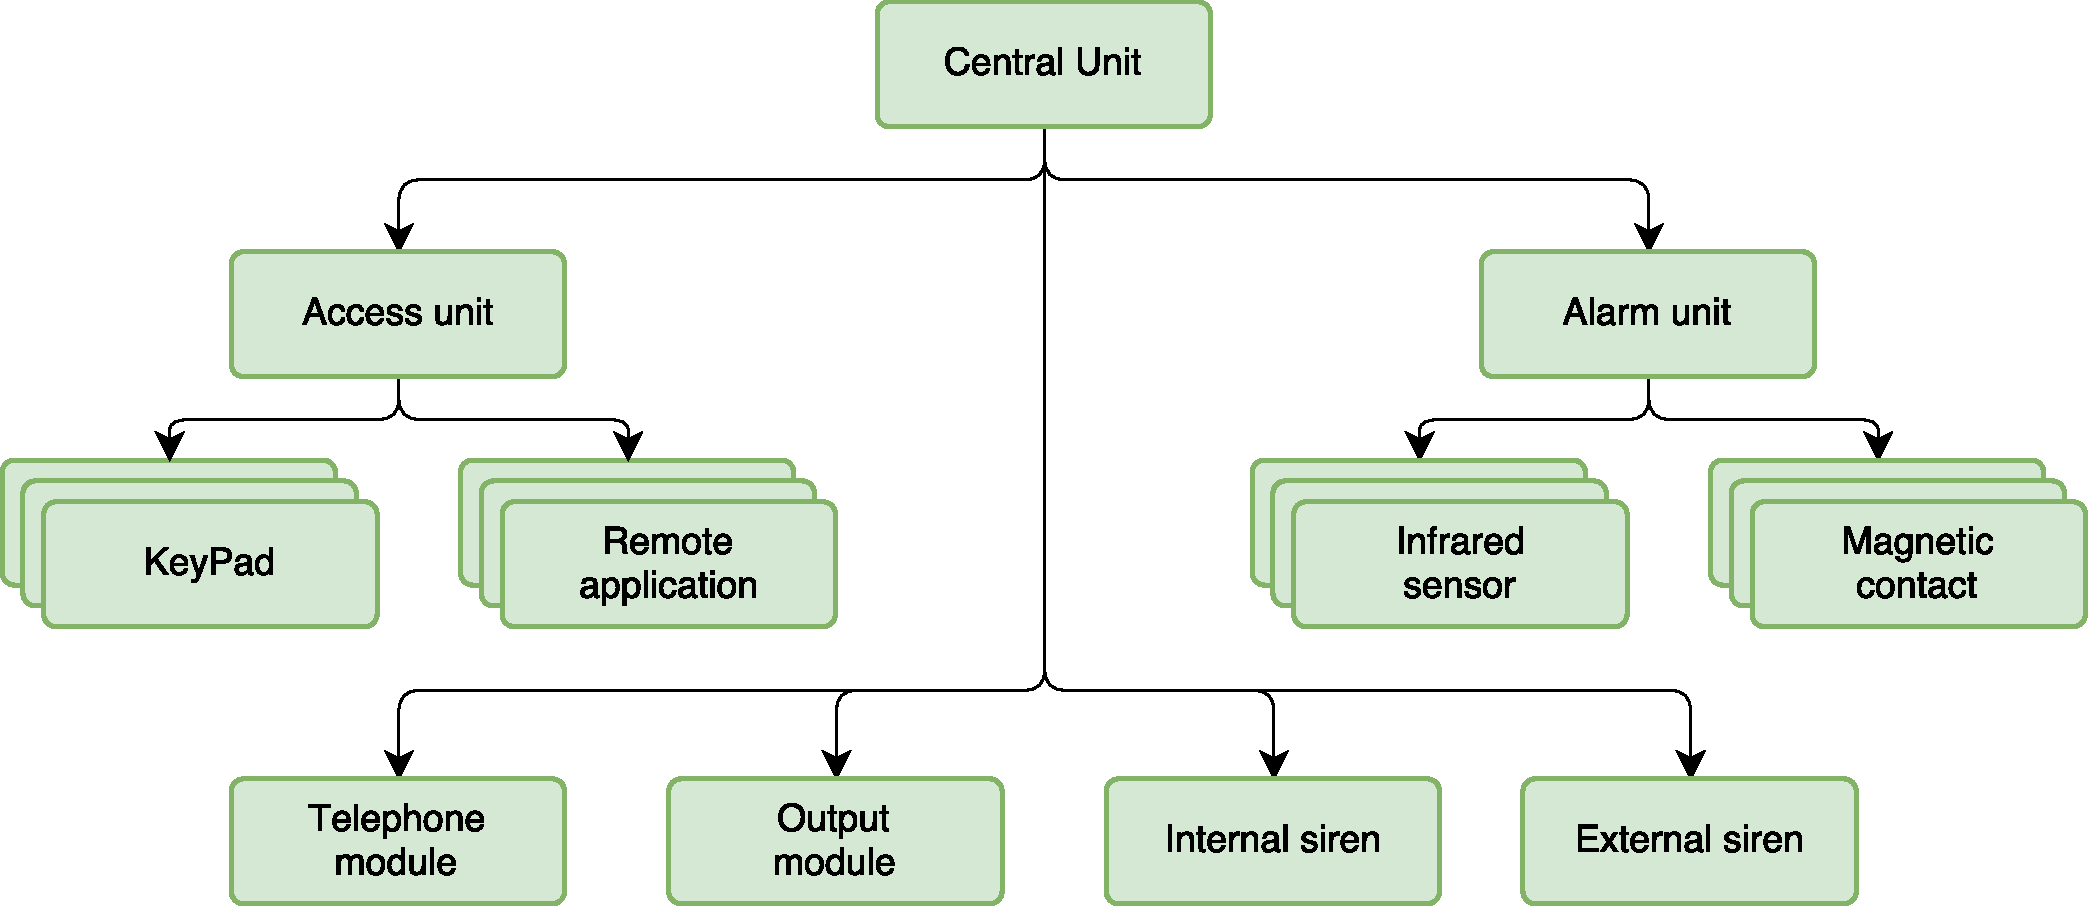
\includegraphics[width=120mm]{images/fmea_structure_definition.pdf}
      \label{fig:fmea_structure_definition}
    \end{figure}
\end{frame}

%%%%%%%%%%%%%%%%%%%%%%
\begin{frame}{FMEA - Change system state}

    \begin{figure}[ht!]
      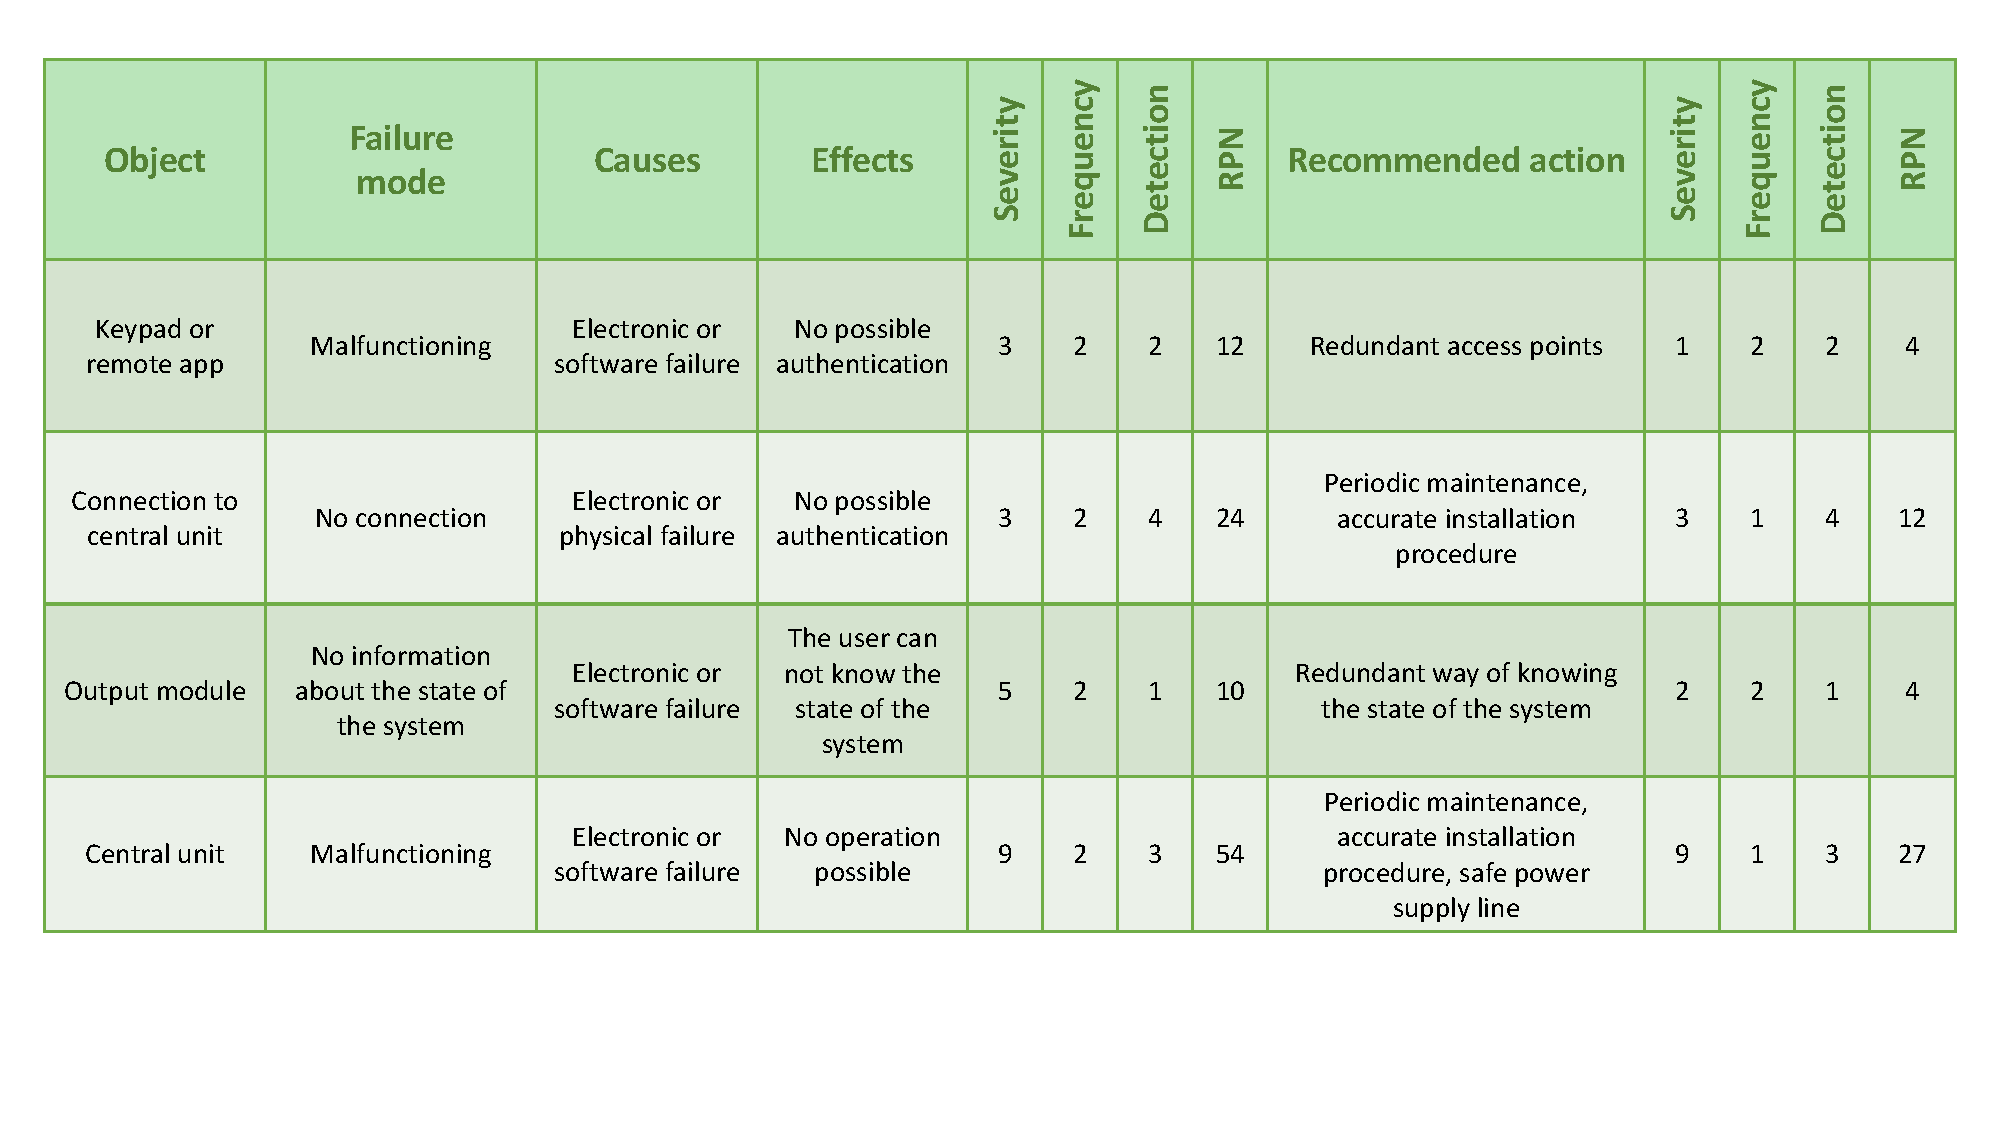
\includegraphics[width=120mm]{images/fmea_change_state.pdf}
      \label{fig:fmea_change_state}
    \end{figure}
\end{frame}

%%%%%%%%%%%%%%%%%%%%%%
\begin{frame}{FMEA - Intrusion detection}
      \vskip 1.0cm
    \begin{figure}[ht!]
      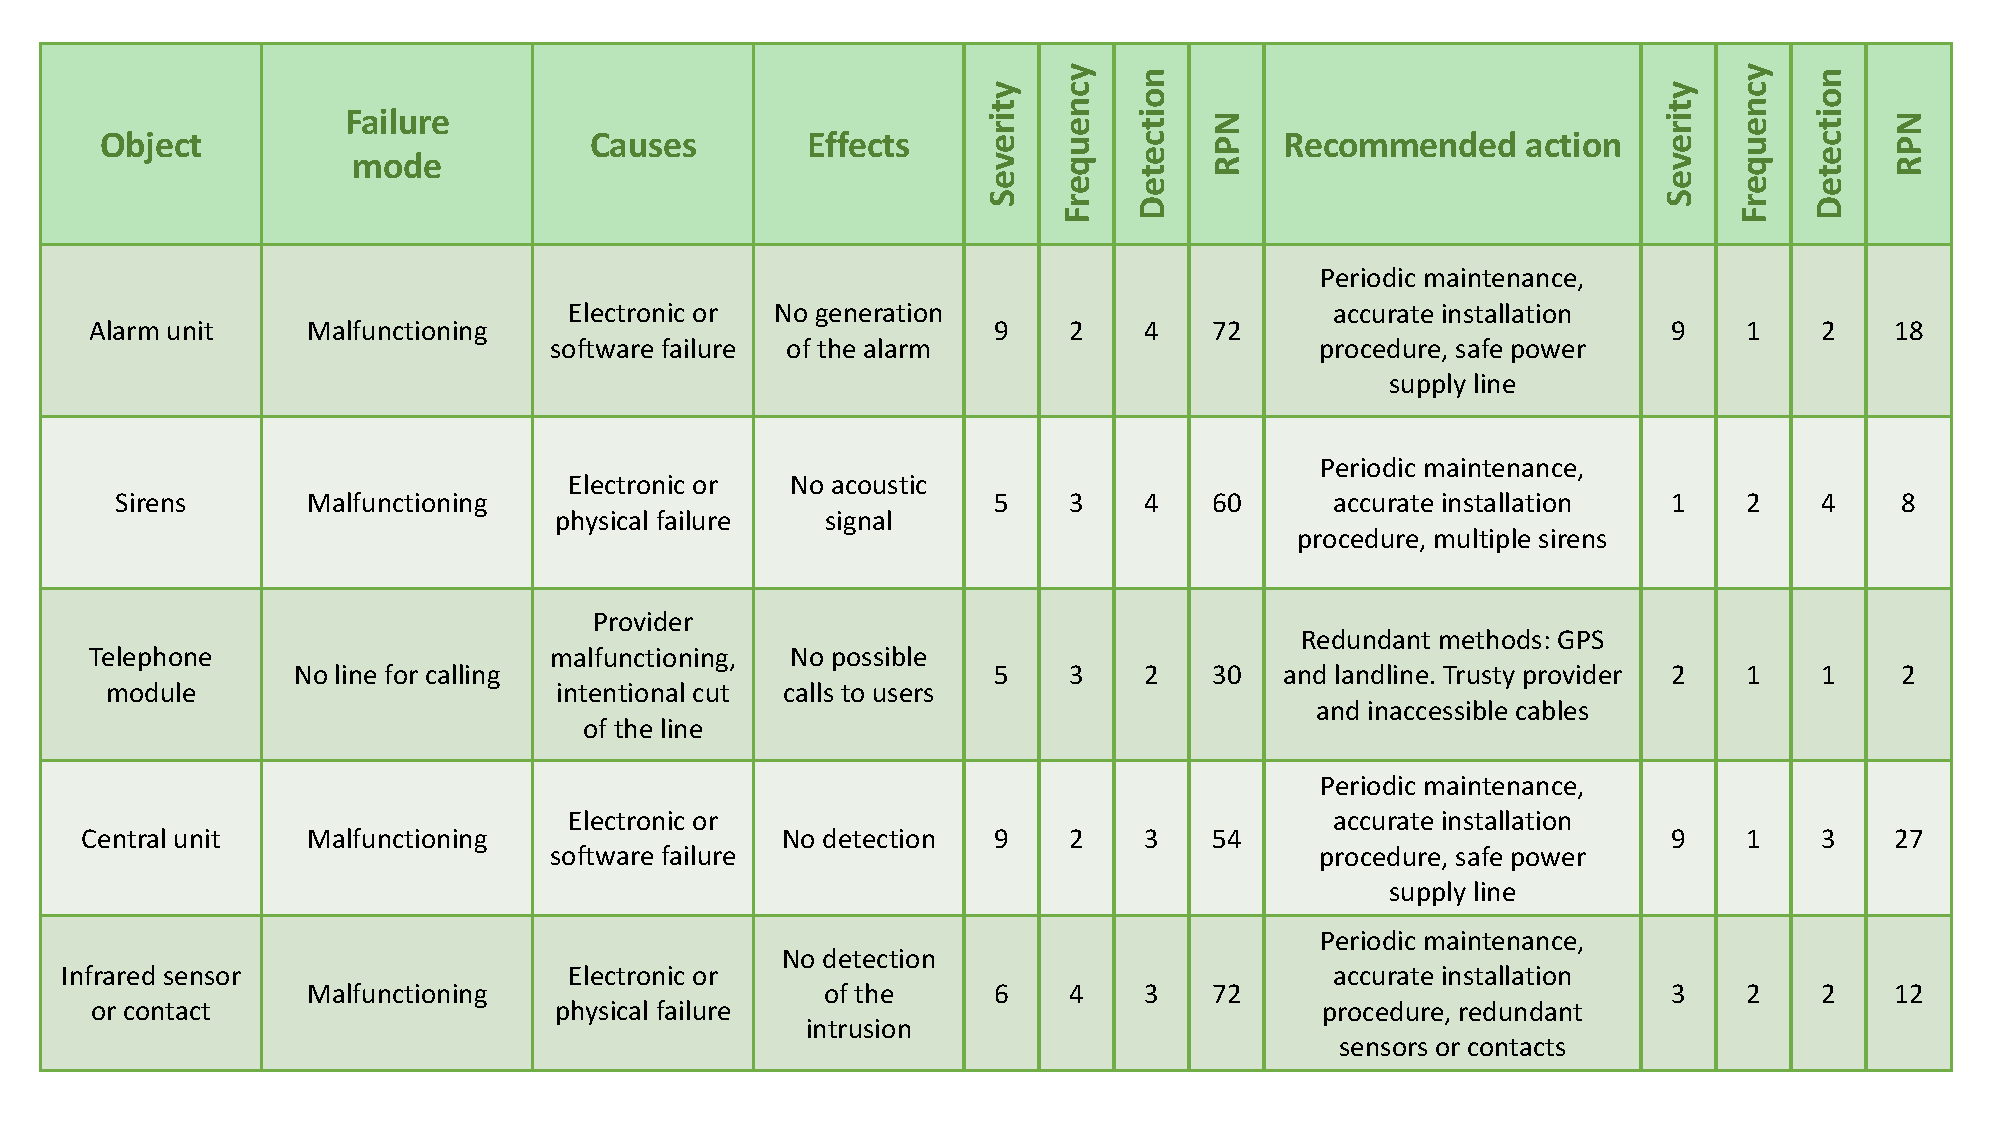
\includegraphics[width=120mm]{images/fmea_intrusion_detection.pdf}
      \label{fig:fmea_intrusion_detection}
    \end{figure}
\end{frame}

%%%%%%%%%%%%%%%%%%%%%%
\begin{frame}{FMEA - System not active}
      \vskip 1.0cm
    \begin{figure}[ht!]
      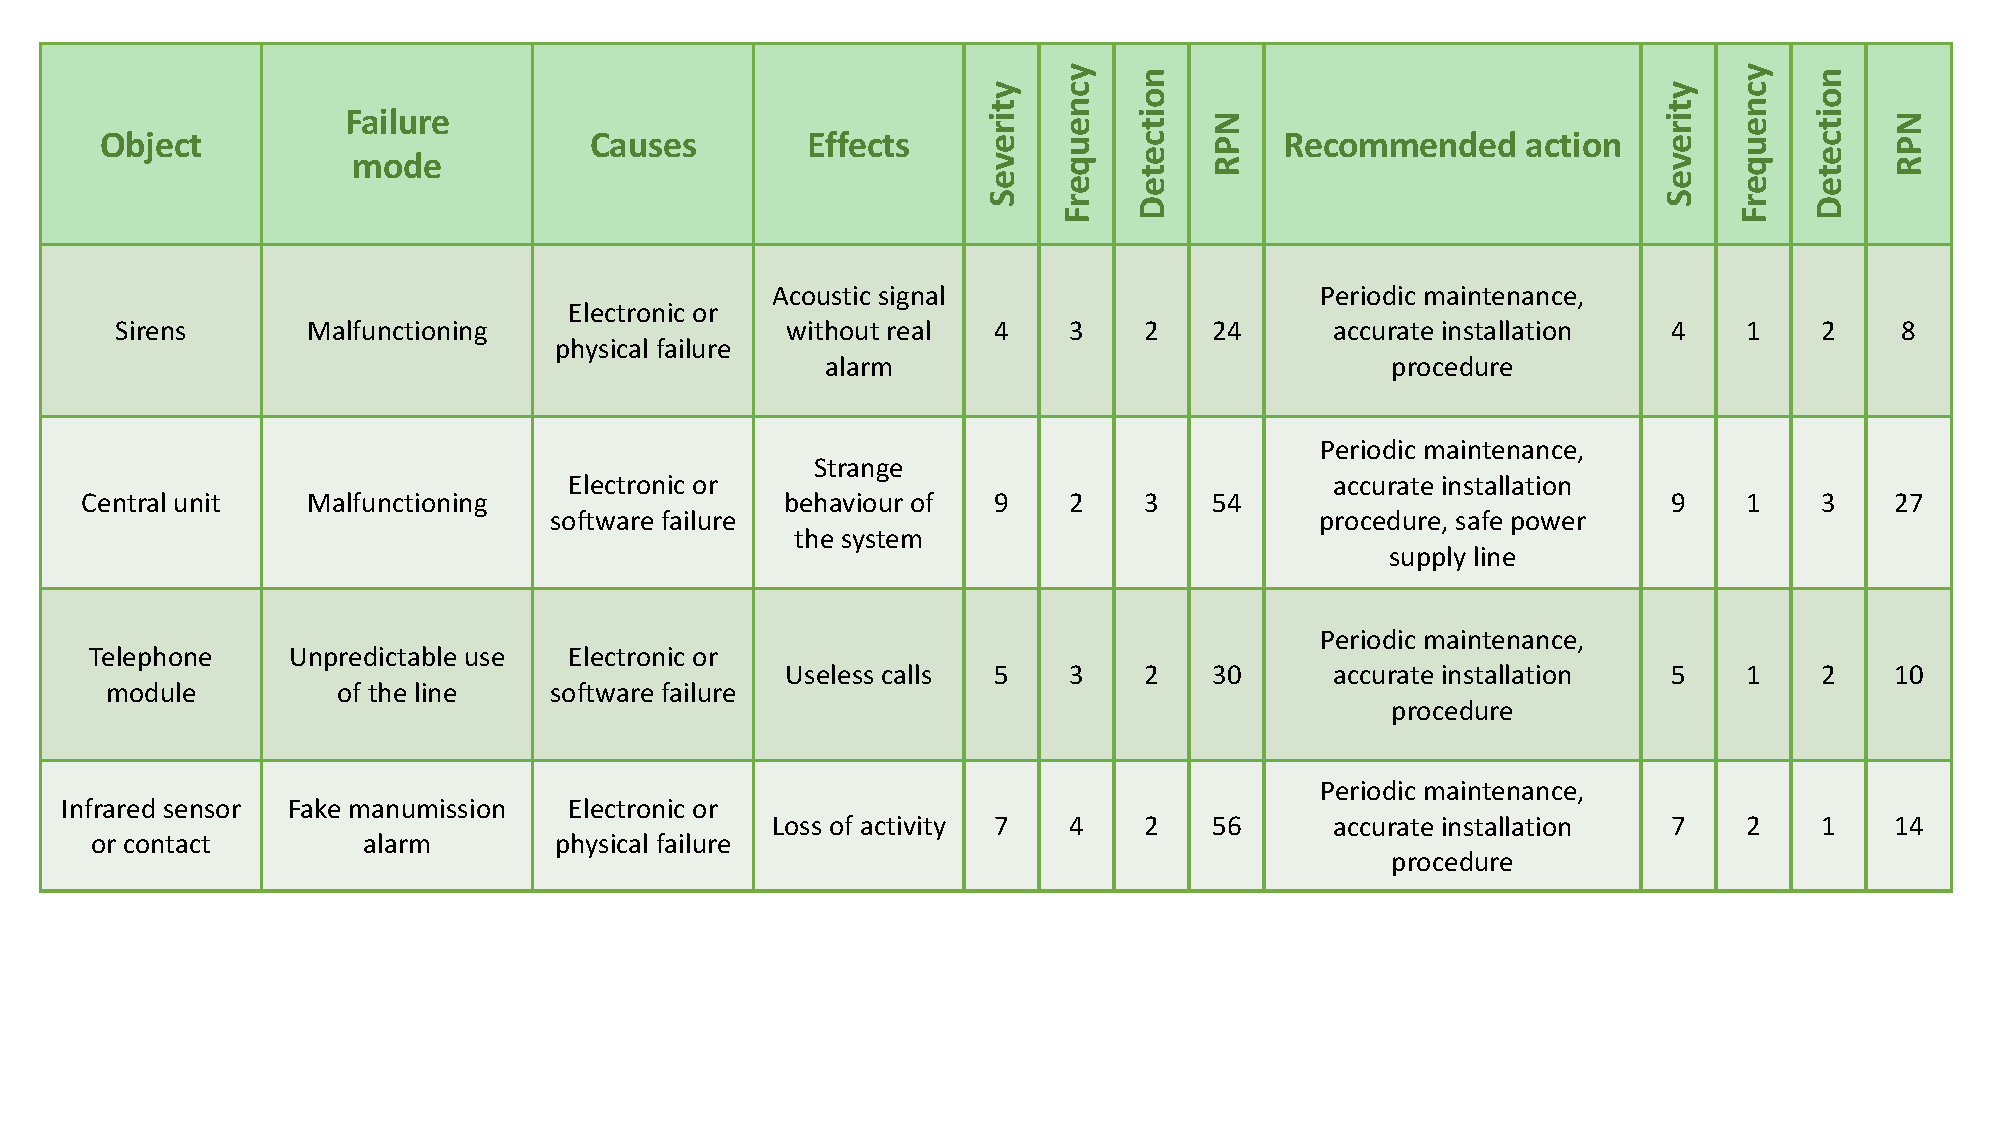
\includegraphics[width=120mm]{images/fmea_system_not_active.pdf}
      \label{fig:fmea_system_not_active}
    \end{figure}
\end{frame}


\subsection{FTA}
\label{sec:fta}
%%%%%%%%%%%%%%%%%%%%%%
\begin{frame}{FTA - Undetected intrusion}

    \begin{figure}[ht!]
      \label{fig:fta_undetected_intrusion}
      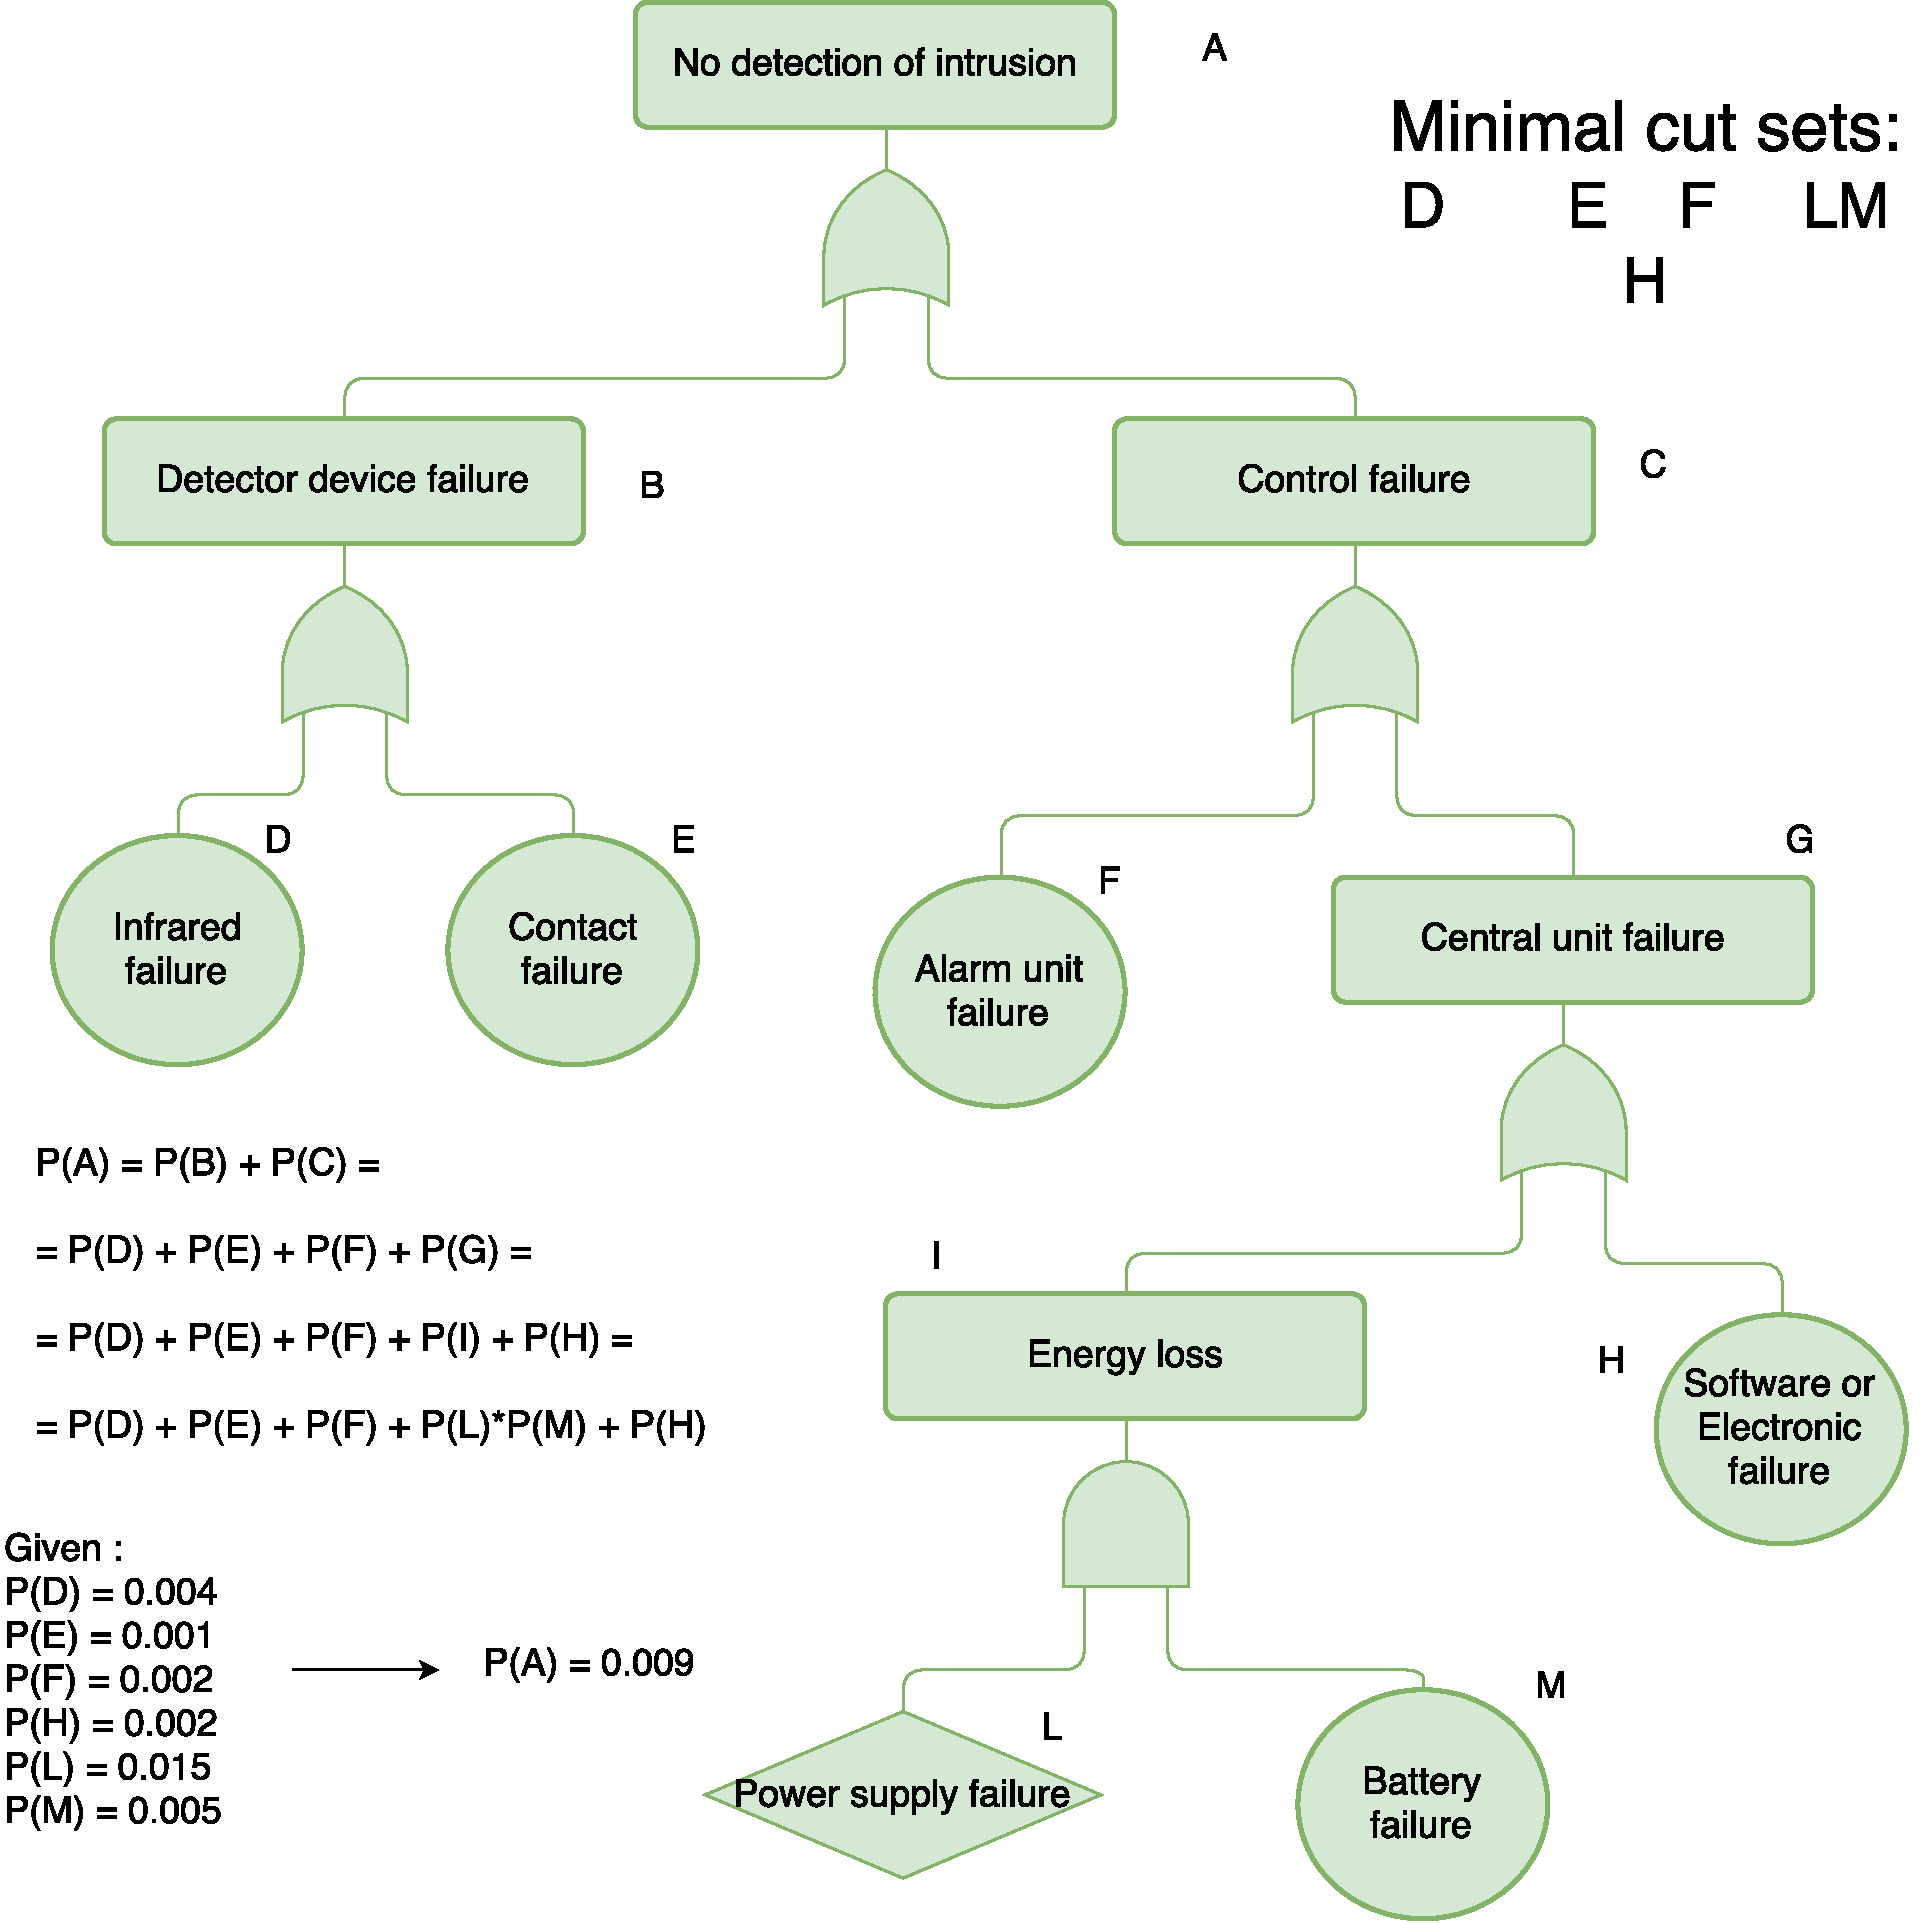
\includegraphics[width=80mm]{images/fta_undetected_intrusion.pdf}
    \end{figure}
\end{frame}

%%%%%%%%%%%%%%%%%%%%%%
\begin{frame}{FTA - No alarm notification}
    \begin{figure}[ht!]
      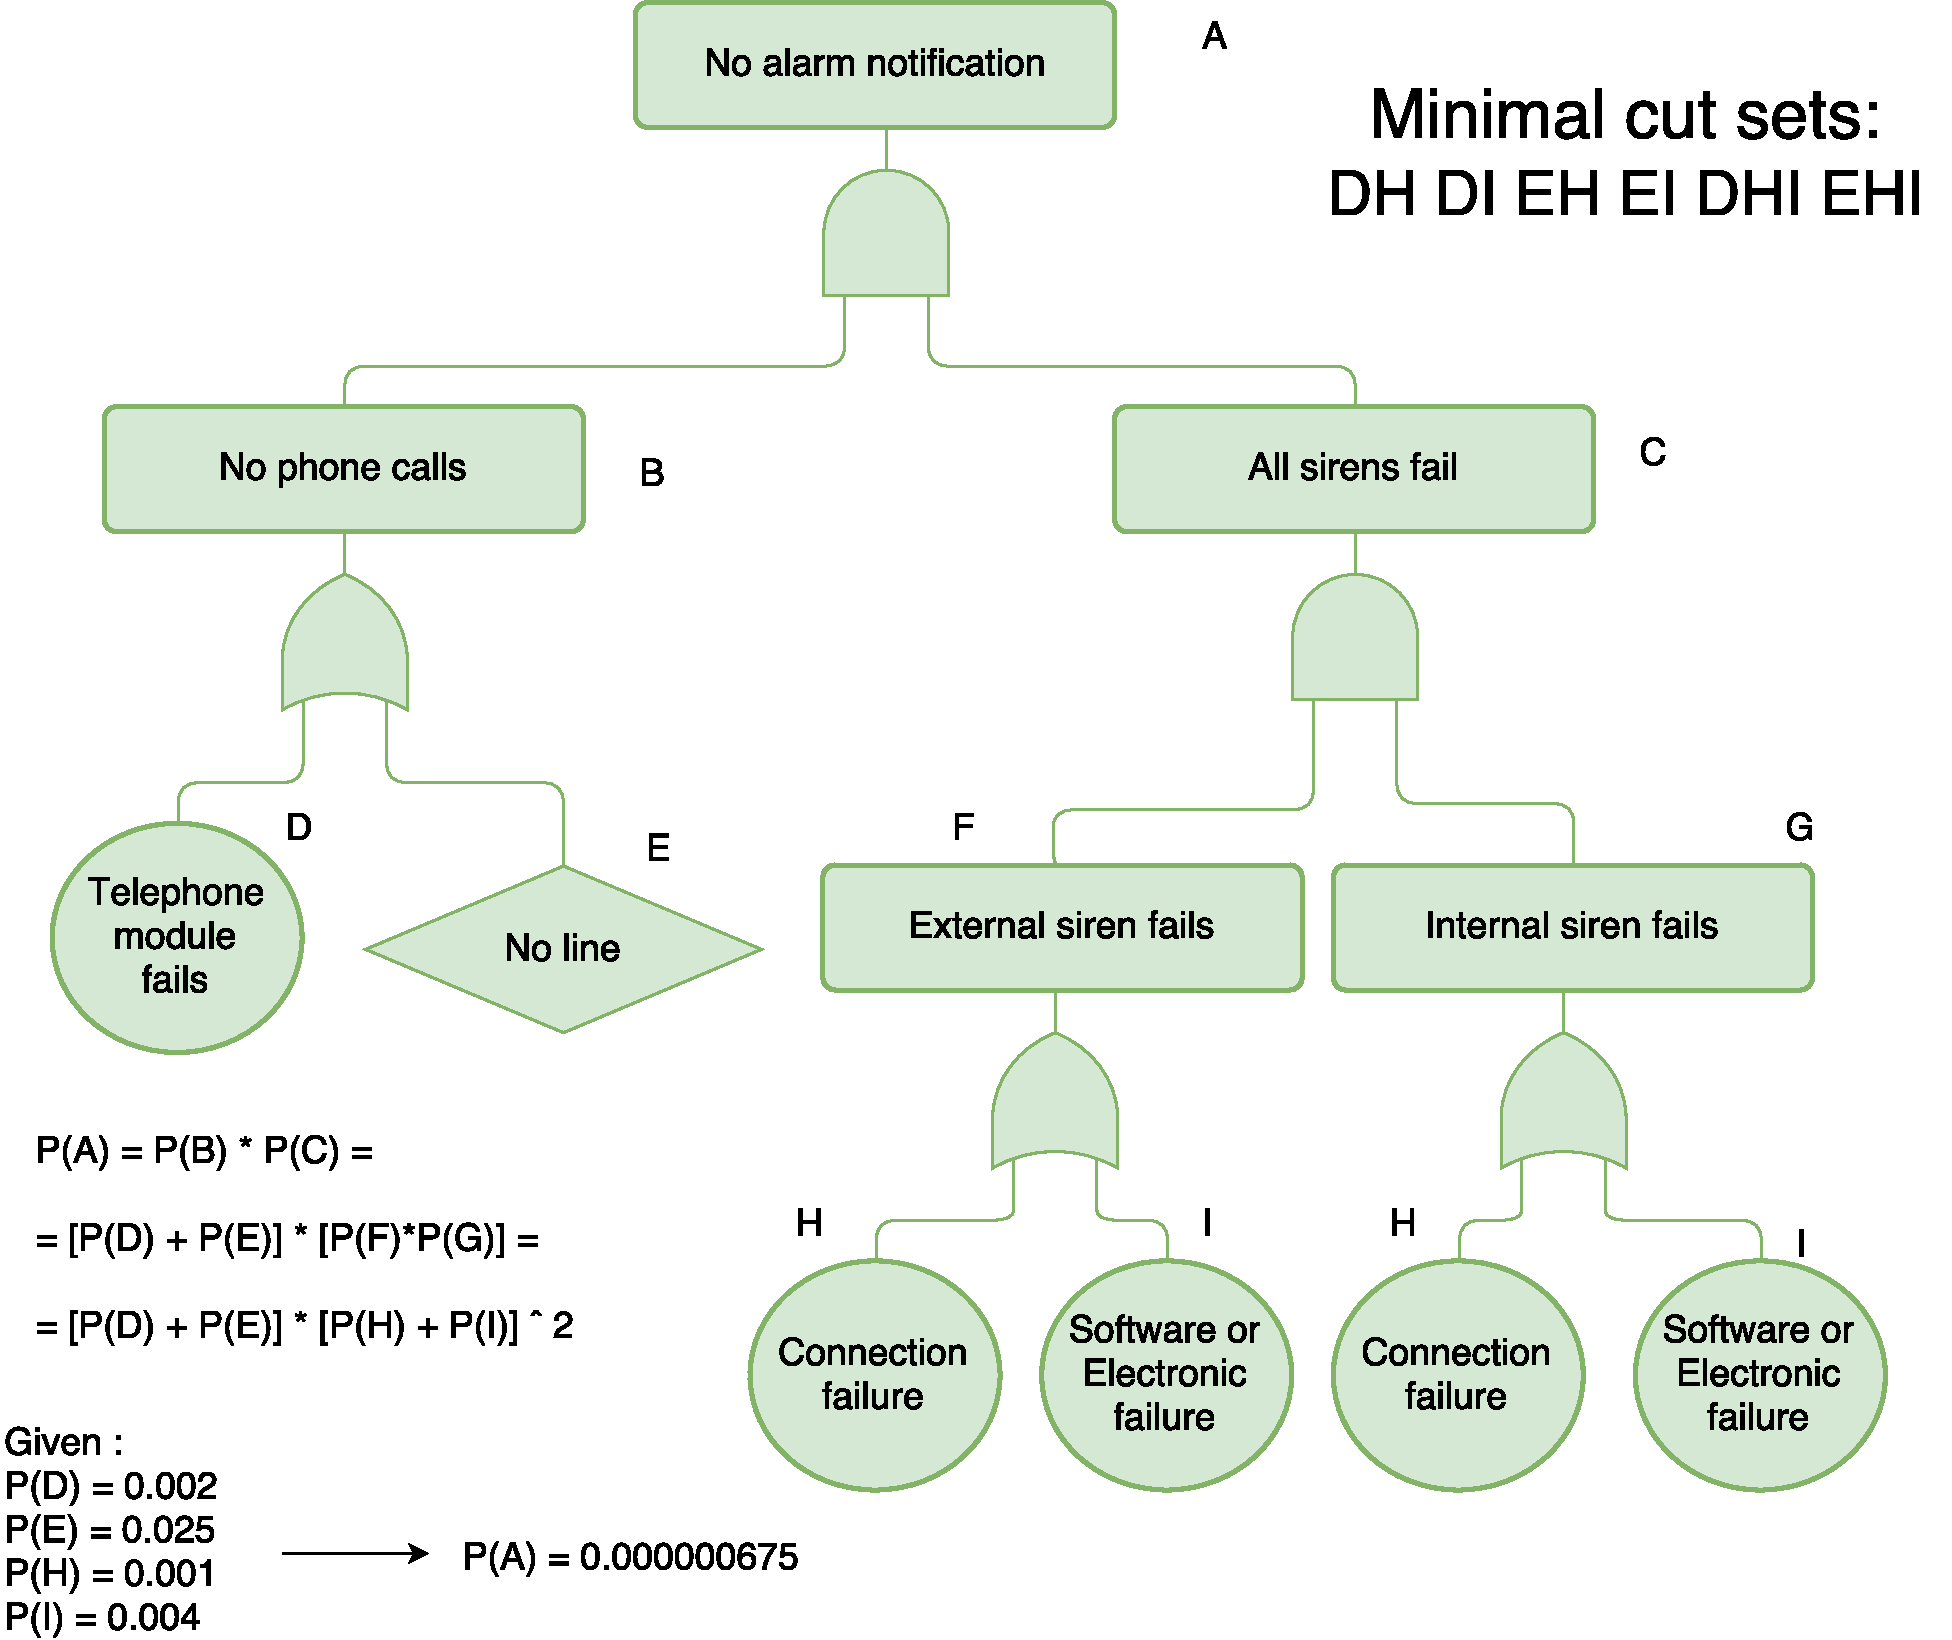
\includegraphics[width=83mm]{images/fta_no_alarm_notification.pdf}
      \label{fig:fta_no_alarm_notification}
    \end{figure}
\end{frame}

%%%%%%%%%%%%%%%%%%%%%%
\begin{frame}{FTA - No change of the system state}
    \begin{figure}[ht!]
      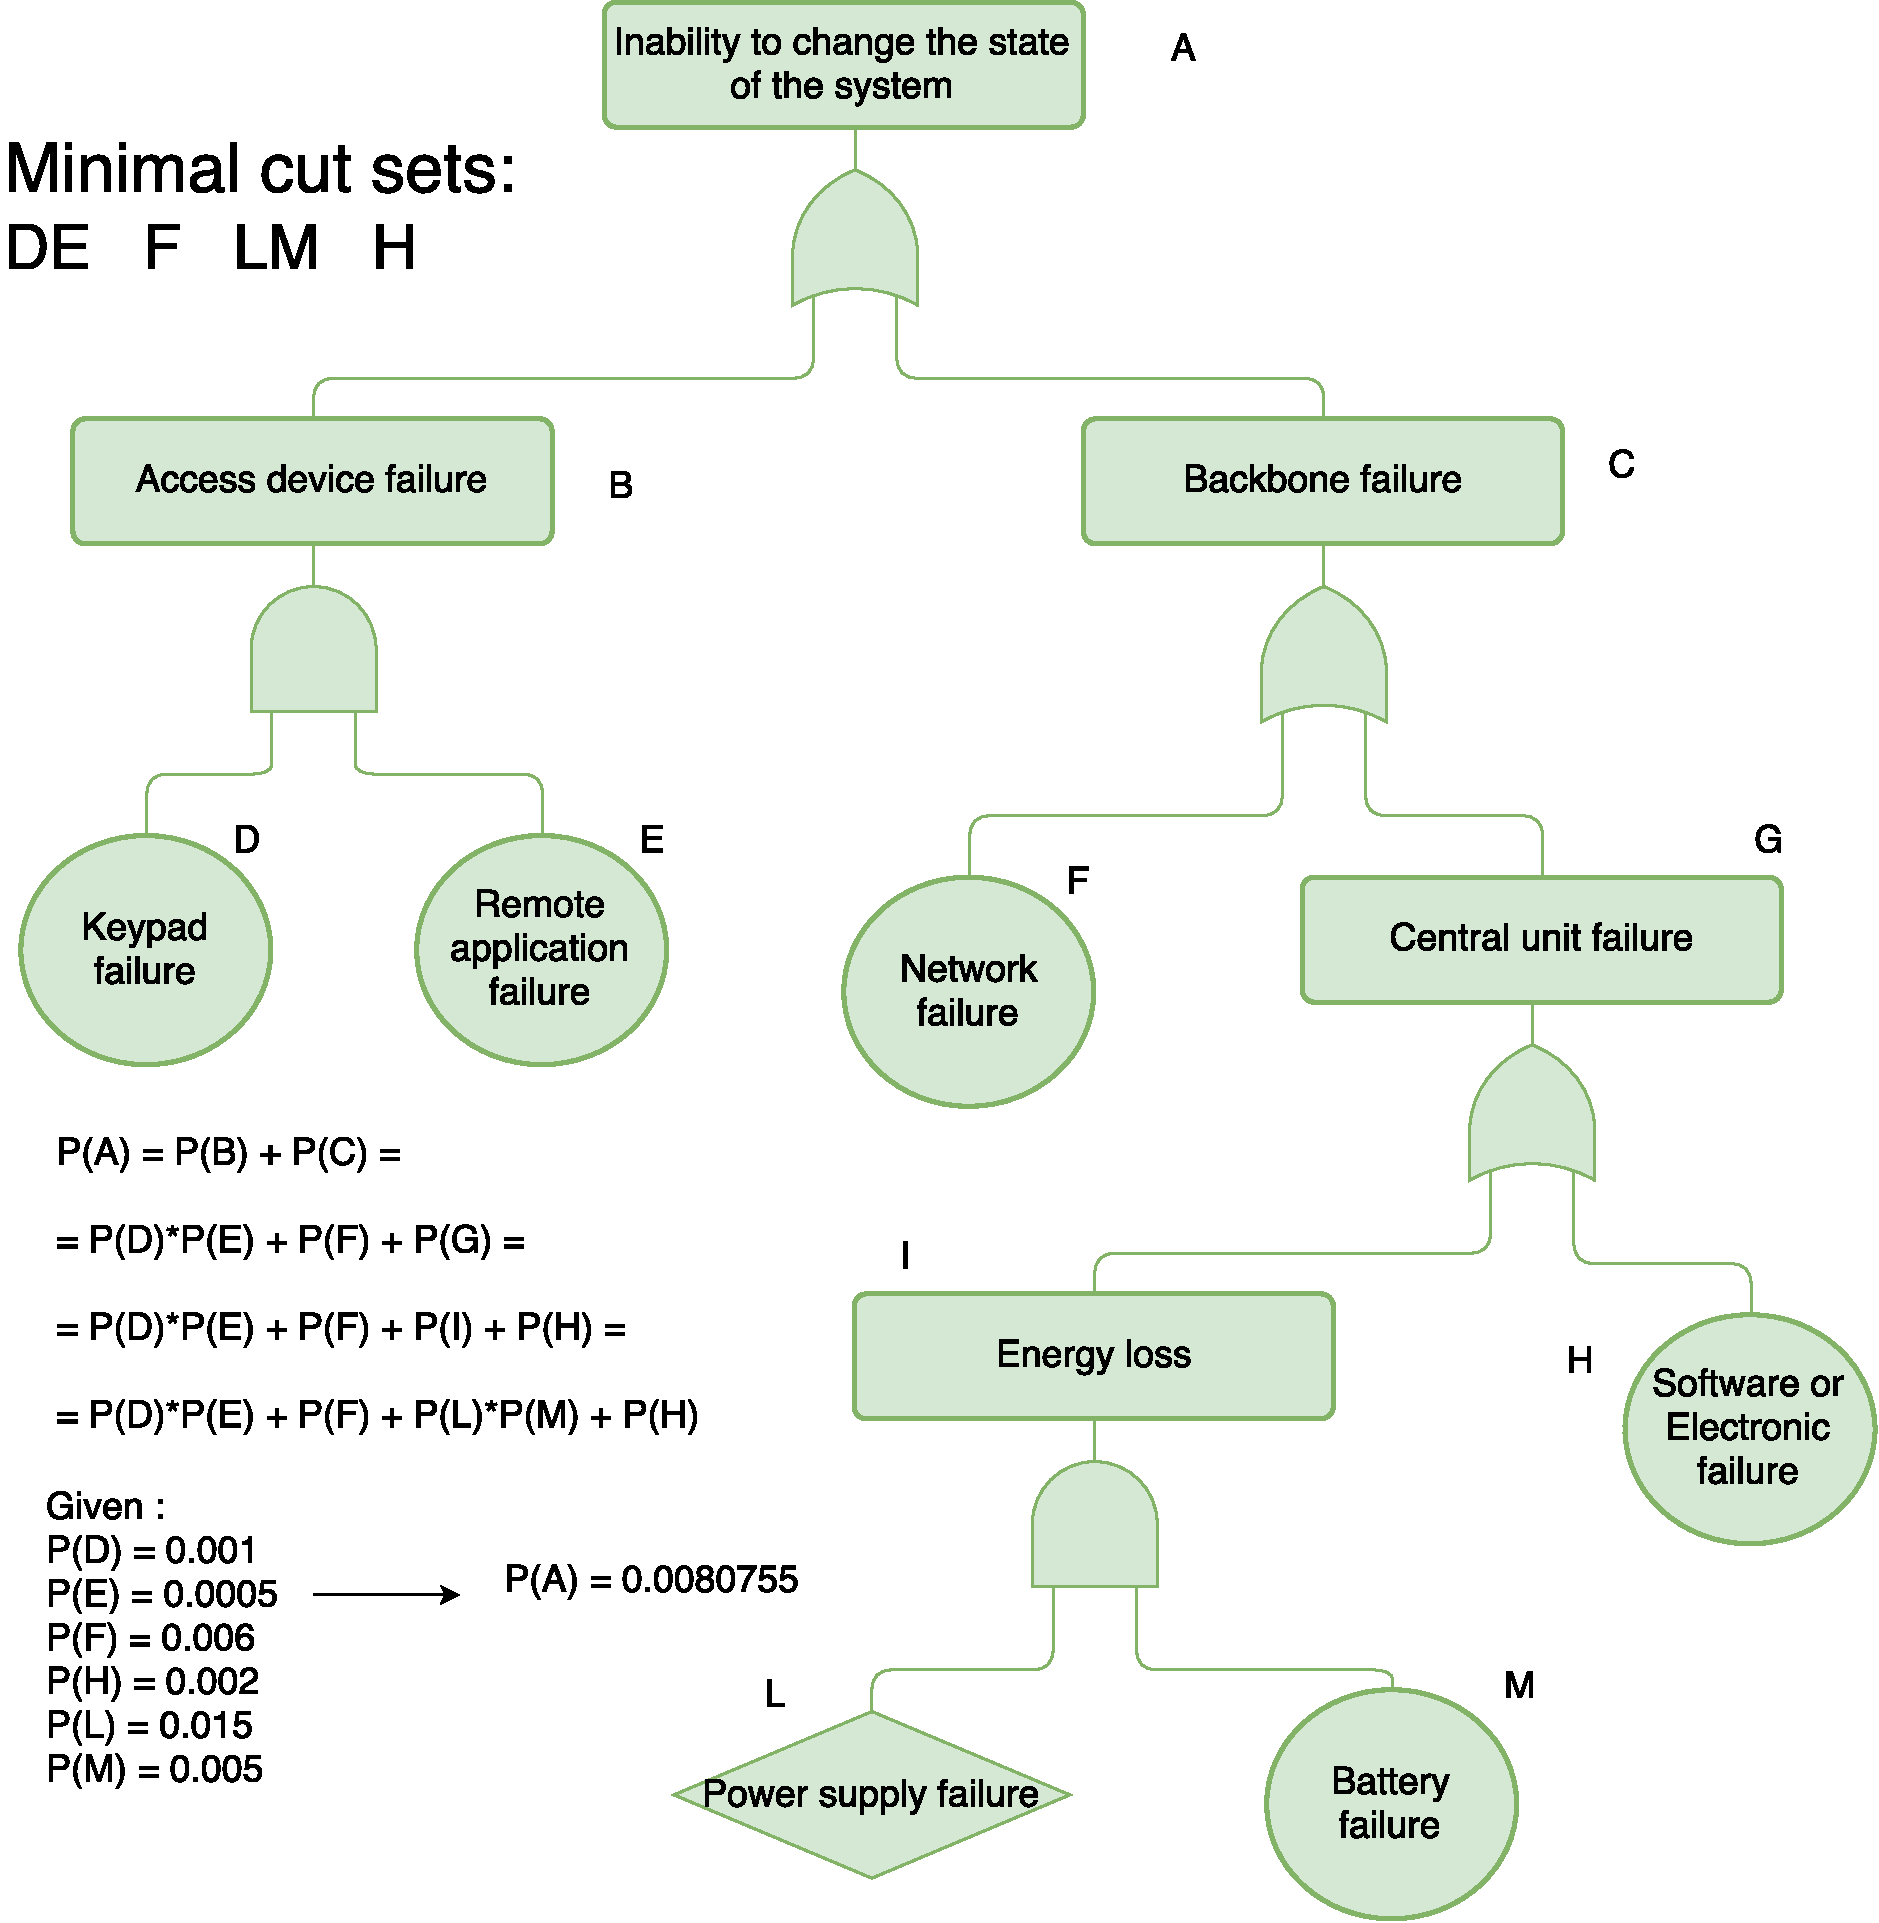
\includegraphics[width=75mm]{images/fta_no_change.pdf}
      \label{fig:fta_no_change}
    \end{figure}
\end{frame}


\subsection{TTM}
\label{sec:ttm}
%%%%%%%%%%%%%%%%%%%%%%
\begin{frame}{TTM - Undetected intrusion}
  \vskip 0.3cm
    The following table refers to FTA - Undetected intrusion.

    1 indicates failure of the component.
    \vskip 0.05cm
    \begin{figure}[ht!]
      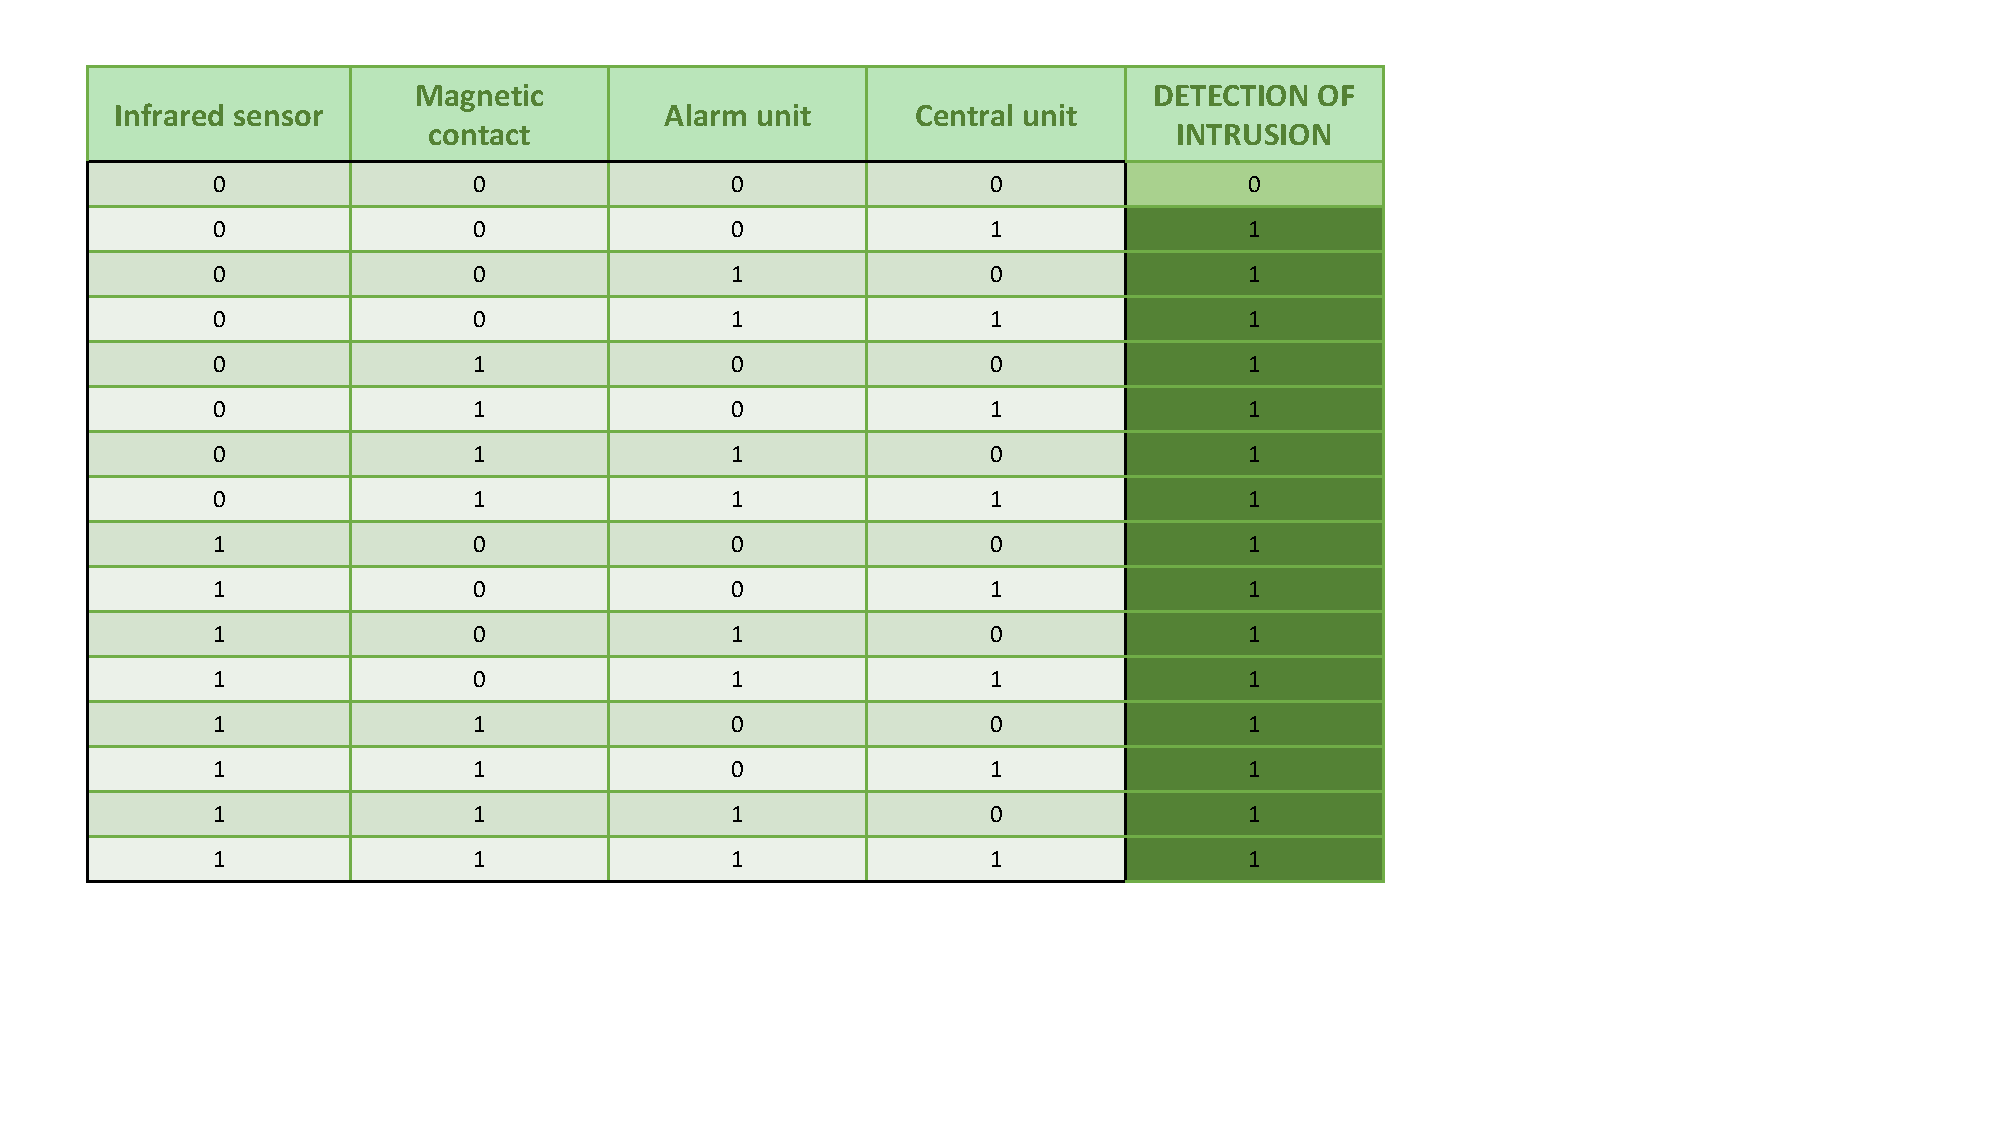
\includegraphics[width=100mm]{images/ttm_undetected_intrusion.pdf}
      \label{fig:ttm_undetected_intrusion}
    \end{figure}
\end{frame}

%%%%%%%%%%%%%%%%%%%%%%
\begin{frame}{TTM - No alarm notification}
  \vskip 0.3cm
    The following table refers to FTA - No alarm notification.

    1 indicates failure of the component.
    \vskip 0.05cm
    \begin{figure}[ht!]
      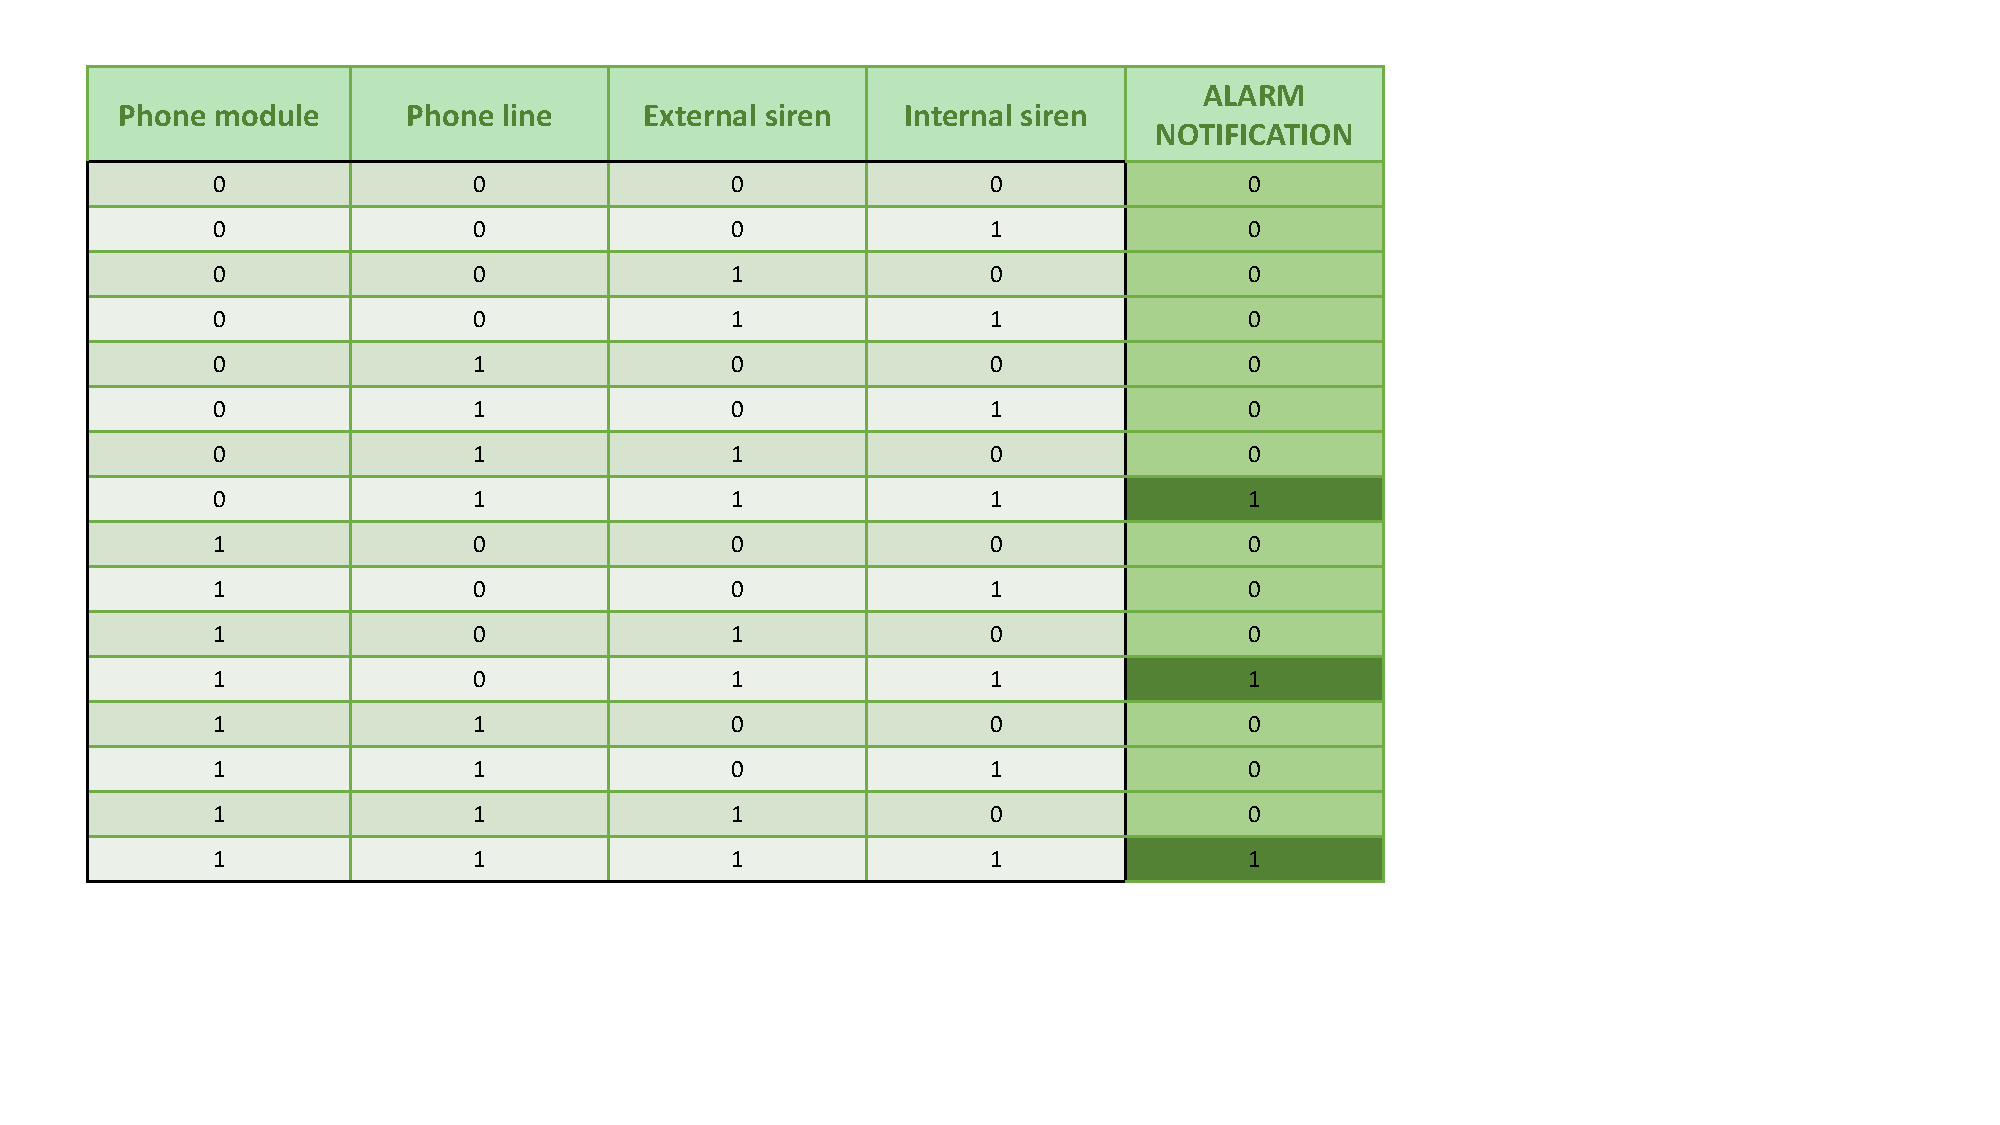
\includegraphics[width=100mm]{images/ttm_alarm_notification.pdf}
      \label{fig:ttm_alarm_notification}
    \end{figure}
\end{frame}

%%%%%%%%%%%%%%%%%%%%%%
\begin{frame}{TTM - No change of the system state}
  \vskip 0.3cm
    The following table refers to FTA - No change of the system

    state. 1 indicates failure of the component.
    \vskip 0.05cm
    \begin{figure}[ht!]
      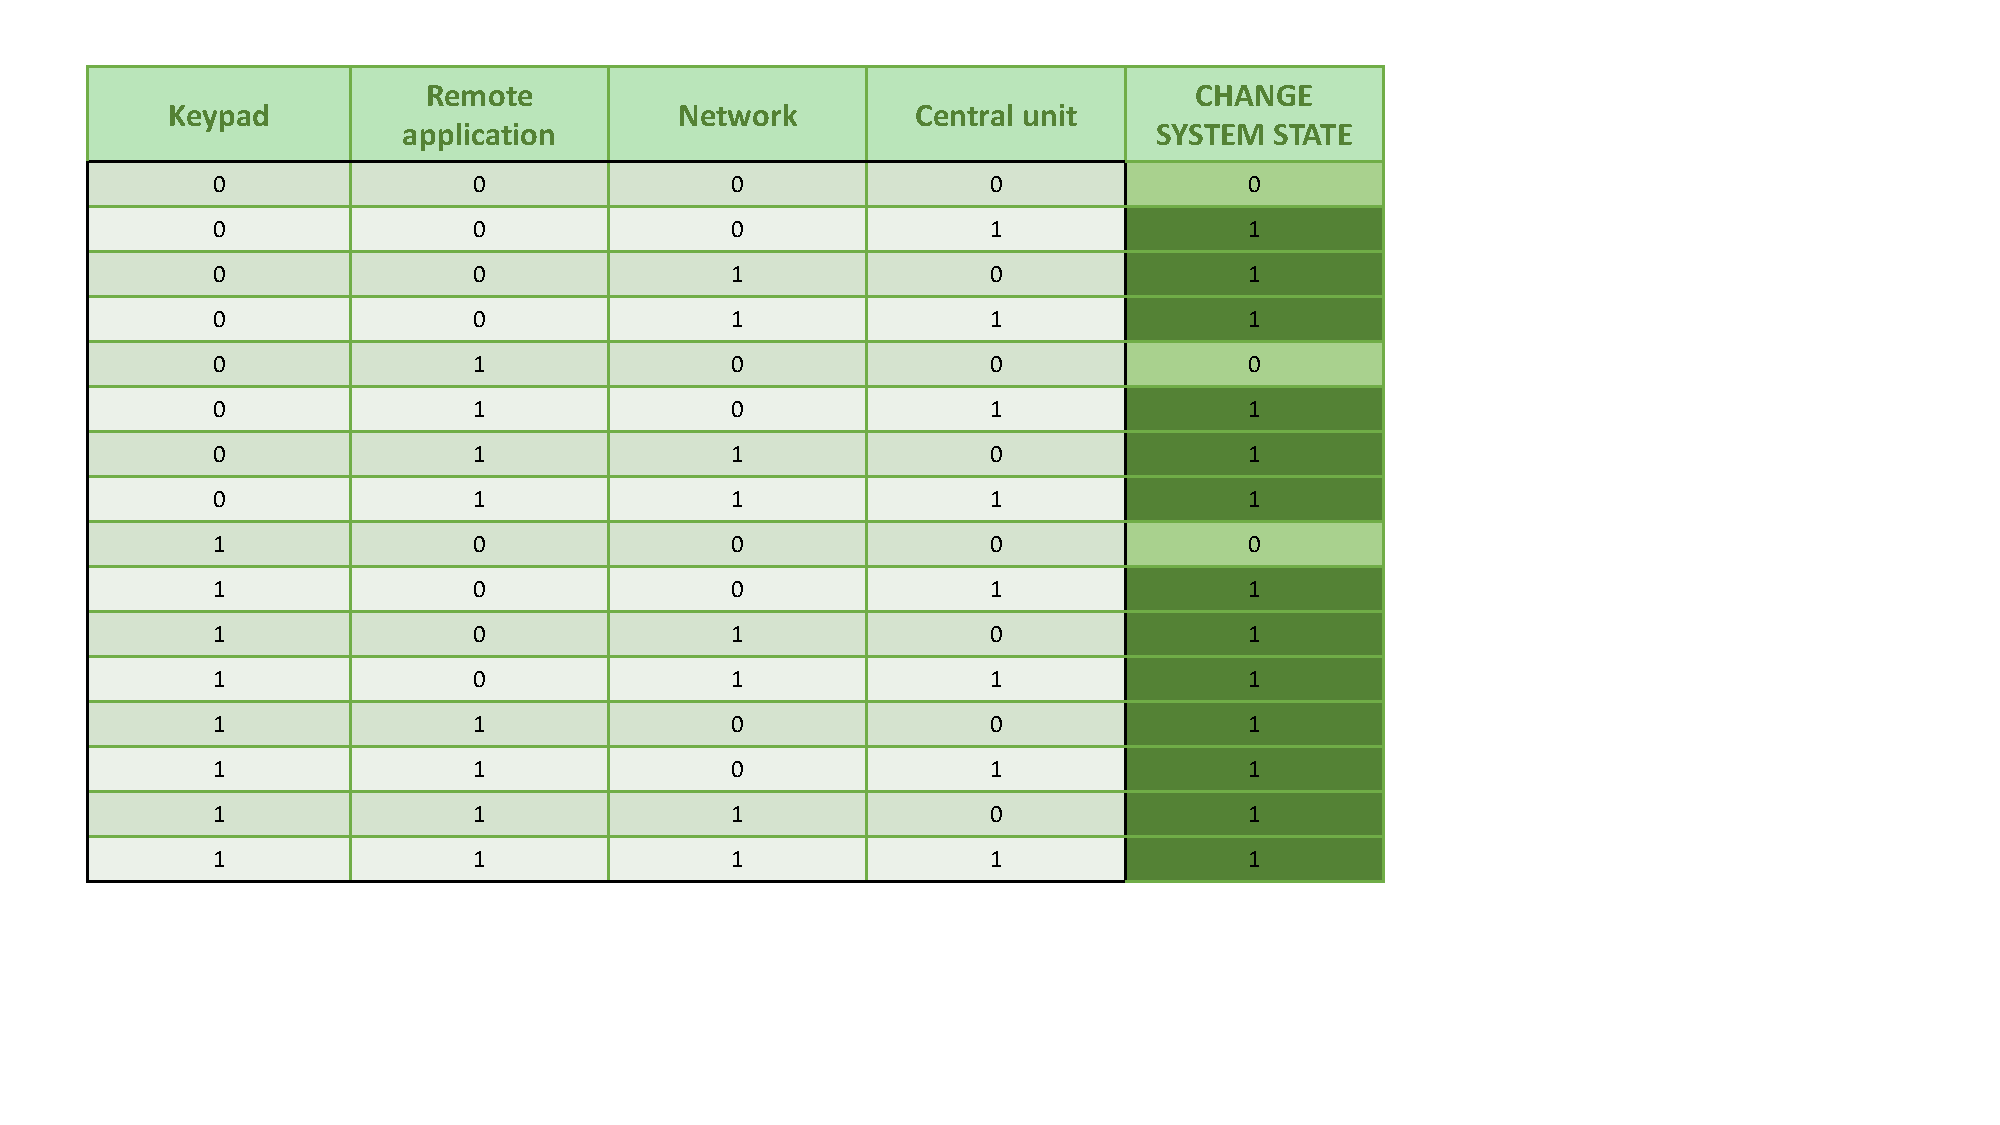
\includegraphics[width=100mm]{images/ttm_no_change_of_the_system_state.pdf}
      \label{fig:ttm_no_change_of_the_system_state}
    \end{figure}
\end{frame}


\subsection{ET}
\label{sec:et}
%%%%%%%%%%%%%%%%%%%%%%
\begin{frame}{ET - User interaction}
  \vskip 0.3cm
    {\textcolor{green!40!black}{\fontsize{13}{15}\textbf{Initiating event: keypad stops working}}}

    The user has to access with the remote application.

    The user also needs the feedback from the
    output module in order to know if the operation was successful or not.
  \vskip 0.4cm
    \begin{figure}[ht!]
      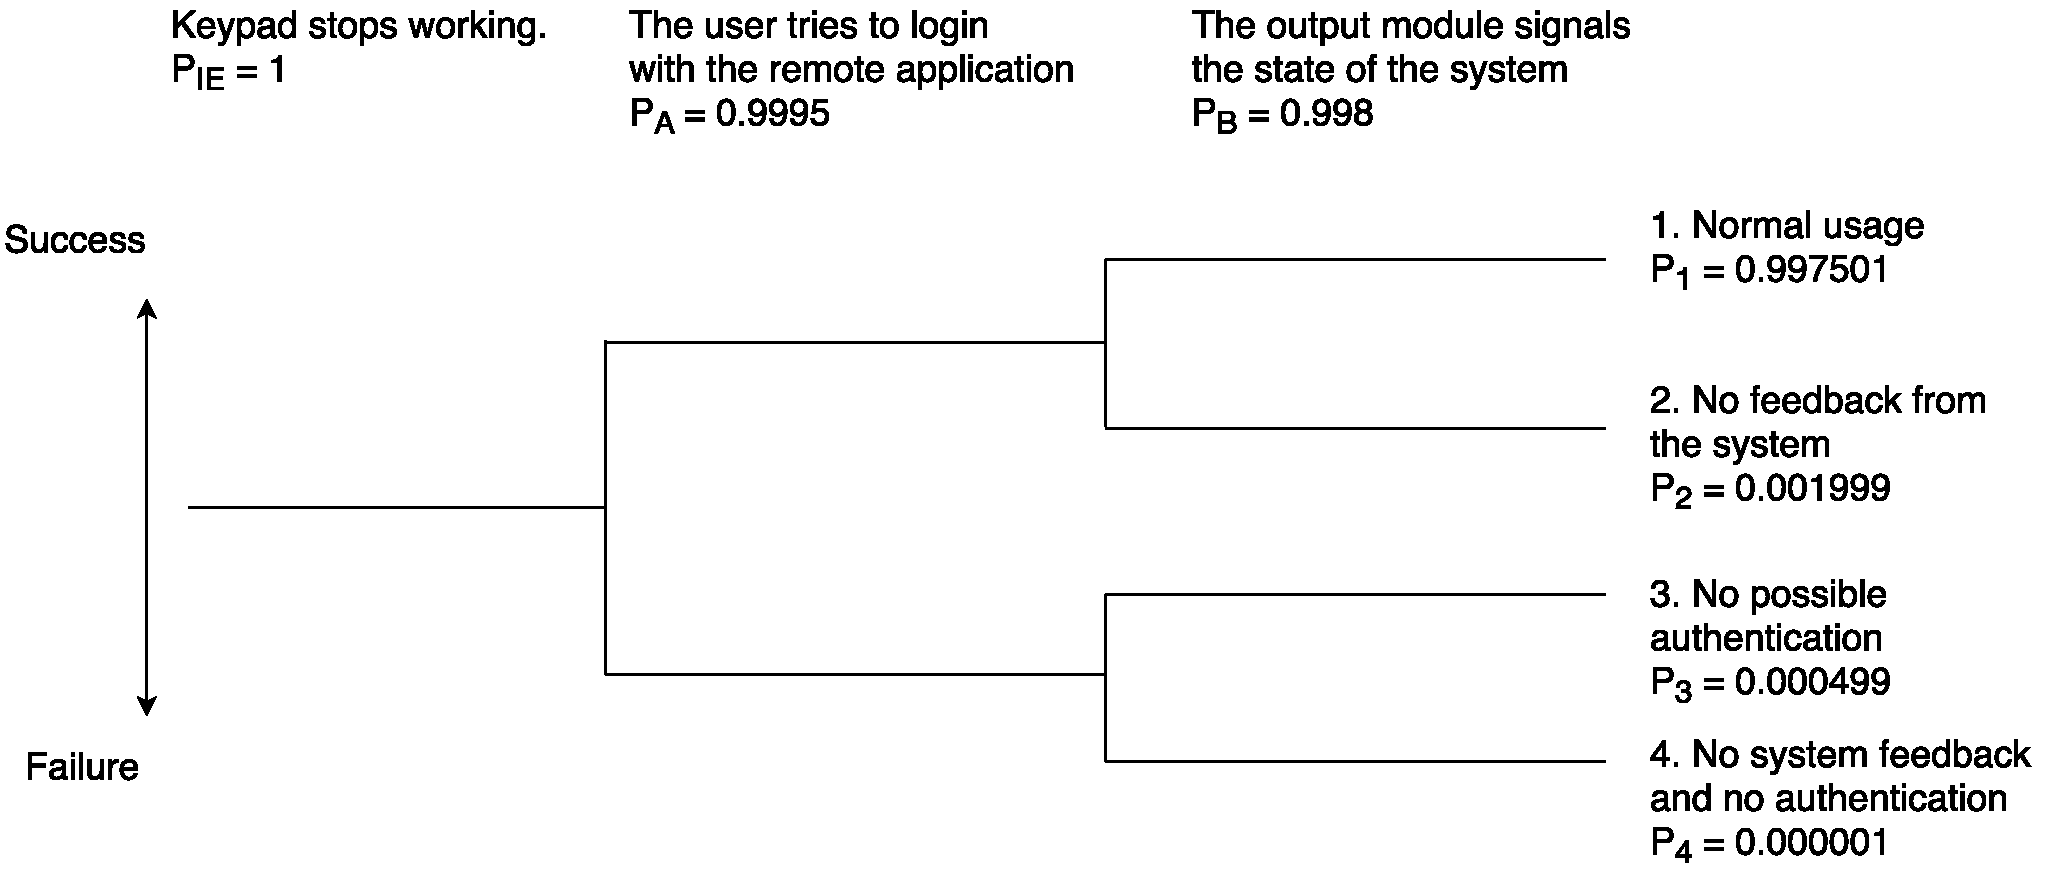
\includegraphics[width=110mm]{images/et_user_interaction.pdf}
      \label{fig:et_user_interaction}
    \end{figure}
\end{frame}

%%%%%%%%%%%%%%%%%%%%%%
\begin{frame}{ET - Intrusion notification}
  \vskip 0.3cm
    {\textcolor{green!40!black}{\fontsize{13}{15}\textbf{Initiating event: sensor stops working}}}

    The system needs to detect the intrusion and notify it locally or remotly.
    \vskip 0.4cm
    \begin{figure}[ht!]
      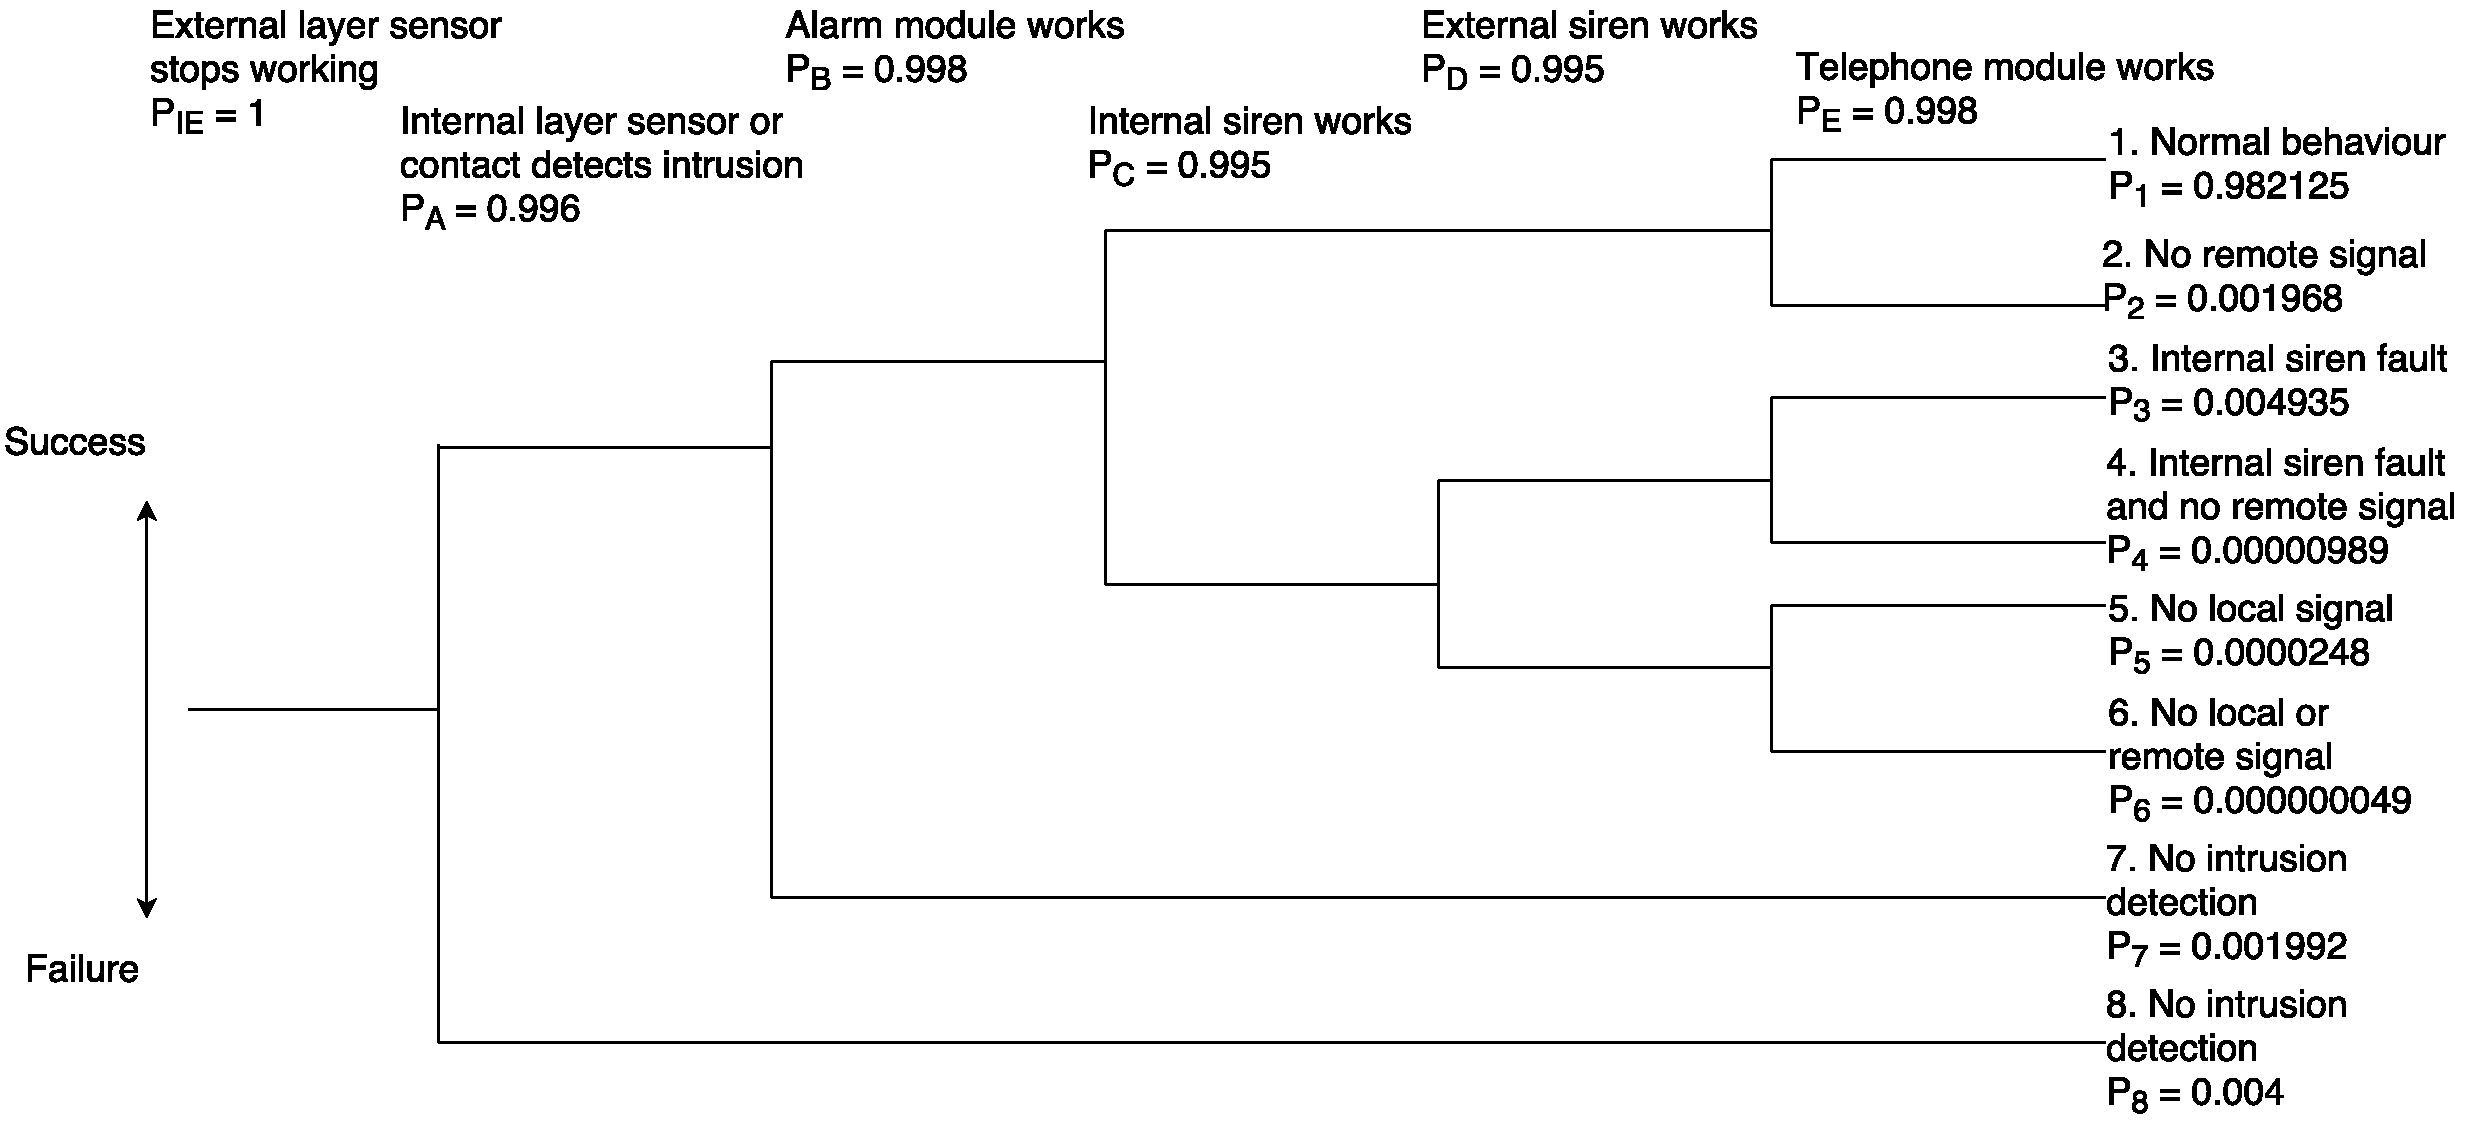
\includegraphics[width=120mm]{images/et_alarm_generation.pdf}
      \label{fig:et_alarm_generation}
    \end{figure}
\end{frame}




%%%%% BIBLIOGRAPHY %%%%%
\begin{frame}{References}
\begin{thebibliography}{9}
\setbeamertemplate{bibliography item}[online]
\bibitem{A} \textbf{Beep - [2016-2017] - SAFETY IN AUTOMATION SYSTEMS} - Riccardo Scattolini -
				\url{https://beep.metid.polimi.it/}
\setbeamertemplate{bibliography item}[online]
\bibitem{B} \textbf{Tecnoalarm systems} - Design of the system
				\url{http://www.tecnoalarm.com/en-uk/installatore/}
\setbeamertemplate{bibliography item}[online]
\bibitem{C} \textbf{Latex} - Document preparation system
				\url{https://www.latex-project.org}


\end{thebibliography}
\end{frame}


%%%%%% END %%%%%%%%%%%
\end{document}
